%%%%%%%%%%%%%%%%%%%%%%%%%%%%%%%%%%%%%%%%%%%%%%%%%%%%%%%%%%%%%%%%%%%%%%
% Lớp 10 | Mệnh đề. Tập hợp | Tập hợp
% Dạng 0D1?2-1: Tập hợp và phần tử của tập hợp
% Số câu: 117  (sinh tự động bởi tach_cau.py; từ nay thầy sửa trực tiếp file này)
%%%%%%%%%%%%%%%%%%%%%%%%%%%%%%%%%%%%%%%%%%%%%%%%%%%%%%%%%%%%%%%%%%%%%%

%%%%%%%%%%%%%%%% TRẮC NGHIỆM 4 PHƯƠNG ÁN %%%%%%%%%%%%%%%%

% nguồn: MaHoaNH_TracNghiem_Lop10
\begin{ex}%[0D1N2-1]%[ma:dea55ae7]
	Trong các tập hợp  sau, tập hợp nào là tập rỗng?
	\choice {$A=\{x\in\mathbb{N}|x^2-4=0\}$}{\True  $B=\{x\in\mathbb{R}|x^2+2x+2025=0\}$}{$C=\{x\in\mathbb{R}|x^2-5=0\}$}{$D=\{x\in\mathbb{Q}|x^2+x-12=0\}$}
	\loigiai{ 
		Phương trình $x^2+2x+2025=0$ vô  nghiệm nên $B=\varnothing$.
	} 
\end{ex}

% nguồn: MaHoaNH_TracNghiem_Lop10
\begin{ex}%[0D1N2-1]%[ma:d1495502]
	Cho tập hợp $B=\{x\in  R|(9-x^{2})(x^{2}-3x+2)=0\}$. Tập hợp nào sau đây là đúng?
	\choice { $B=\{3;9;1;2\}$}{ $B=\{-3;-9;1;2\}$}{\True $B=\{-3;3;1;2\}$}{  $B=\{-9;9;1;2\}$}
	\loigiai{ 
		Ta có $(9-x^{2})(x^{2}-3x+2)=0\Leftrightarrow\heva{&9-x^{2}=0 &\Rightarrow x=\pm3\\& x^{2}-3x+2=0 &\Rightarrow x=1 \text{ hoặc  } x=2.}$\\
		Vậy $B=\{-3;3;1;2\}$. 
	} 
\end{ex}

% nguồn: MaHoaNH_TracNghiem_Lop10
\begin{ex}%[0D1N2-1]%[ma:828015ce]
	Hãy liệt kê các phần tử của tập  hợp$X=\left\{x\in \mathbb{R}\big|x^2+x+1=0\right\}$.
	\choice 
		{$X=0$} 
		 {$X=\left\{0\right\}$}
		{\True  $X=\varnothing $}
		 {$X=\left\{\varnothing\right\}$}
	\loigiai{ 
	Phương  trình $x^2+x+1=0$ vô nghiệm nên $X=\varnothing$.}
\end{ex}

% nguồn: MaHoaNH_TracNghiem_Lop10
\begin{ex}%[0D1N2-1]%[ma:b6ca175f]
	Cho tập hợp $A=[1;5]$, phát biểu nào sau đây đúng? 
	 \choice
		{$A=\{x\in\mathbb{N}\mid  1\le x\le 5\}$}
		{\True$A=\{x\in \mathbb{R}\mid 1\le x\le 5\}$} 
		 {$A=\{1;2;3;4;5\}$}
		{$A=\{1;5\}$} 
	\loigiai{ 
		 Ta có $A=\{x \in \mathbb{R}\mid 1 \le x \le 5\}$.
	} 
\end{ex}

% nguồn: MaHoaNH_TracNghiem_Lop10
\begin{ex}%[0D1N2-1]%[ma:72ce3cad]
	 Cho tập hợp $A=\{x \mid x \in \mathbb{N}, x \leq 5\}$. Số phần tử của tập hợp $A$ là
	 \choice
		{$8$} 
		 {$7$}
		{$5$} 
		{\True  $6$}
	 \loigiai{
		$A=\{x \mid x \in \mathbb{N}, x \leq 5\} \Leftrightarrow A=\{0; 1; 2; 3; 4; 5\}$. Do đó số phần  tử của tập hợp $A$ là $6$.
	} 
\end{ex}

% nguồn: MaHoaNH_TracNghiem_Lop10
\begin{ex}%[0D1N2-1]%[ma:a1a86b2f]
	Ký hiệu nào sau đây đúng khi $\sqrt{5}$ không phải là một số hữu  tỉ?
	 \choice
		{$\sqrt{5} \neq \mathbb{Q}$} 
		{$\sqrt{5}  \subset \mathbb{Q}$}
		{\True $\sqrt{5}  \notin \mathbb{Q}$}
		{$\sqrt{5} \in  \mathbb{Q}$}
	\loigiai{ 
		Vì $\sqrt{5}$ chỉ là một phần tử và $\mathbb{Q}$ là một tập hợp nên các đáp  án $\sqrt{5} \neq \mathbb{Q}$, $\sqrt{5} \subset \mathbb{Q}$, $\sqrt{5} \in \mathbb{Q}$ đều sai.
	 }
\end{ex}

% nguồn: MaHoaNH_TracNghiem_Lop10
\begin{ex}%[0D1N2-1]%[ma:46c80877]
	Hãy viết tập hợp sau bằng cách nêu tính chất đặc trưng cho các phần tử  của tập hợp $A=\{0;4;8;12\}$.
	\choice 
		{$A  = \{ x \in \mathbb{R} \mid x \,\vdots\, 4 \text{\,và\,} x \le 14 \}$}
		{$A = \{ x \in \mathbb{Z} \mid x \,\vdots\, 4 \text{\,và\,} x \le 15 \}$} 
		{\True $A = \{ x  \in \mathbb{N} \mid x \,\vdots\, 4\text{\,và\,} x \le 15 \}$}
		{$A = \{ x \in \mathbb{N} \mid x \,\vdots\, 5  \text{\,và\,} x \le 15 \}$}
	 \loigiai{
		Ta thấy,các phần tử của $A=\{0;4;8;12\}$ chia hết cho $4$ và bé hơn  $15$, nên $A=\{x\in \mathbb{N}\mid x \,\vdots\, 4 \text{\,và\,} x \le 15 \}$.
	 }
\end{ex}

% nguồn: MaHoaNH_TracNghiem_Lop10
\begin{ex}%[0D1N2-1]%[ma:7247cf2f]
	Hãy liệt kê các phần tử của tập hợp $X=\{x\in \mathbb{R}\mid  x^2+x+1=0\}$
	 \choice
		{$X=0$} 
		 {$X=\{0\}$}
		{\True  $X=\varnothing$}
		 {$X=\left\{\varnothing\right\}$}
	\loigiai{ 
		Phương trình $x^2+x+1=0$ vô nghiệm nên  $X=\varnothing$.
	} 
\end{ex}

% nguồn: MaHoaNH_TracNghiem_Lop10
\begin{ex}%[0D1N2-1]%[ma:ad949b37]
	Tập  hợp $A=\{x\in \mathbb{R}\mid 4x+1>10 \}$ bằng tập hợp nào dưới đây?
	\choice 
		 {$\left(\dfrac{9}{4};+\infty\right)$}
		 {$\left(- \dfrac{9}{4};+\infty\right)$}
		{$\left[\dfrac{9}{4};+\infty\right)$} 
		 {\True $\left(\dfrac{9}{4};+\infty\right)$}
	\loigiai{ 
		Ta có $4x+1>10  \Leftrightarrow x\in \left(\dfrac{9}{4};+\infty\right)$.\\
		Vậy $A=\left(\dfrac{9}{4};+\infty\right)$. 
	} 
\end{ex}

% nguồn: MaHoaNH_TracNghiem_Lop10
\begin{ex}%[0D1N2-1]%[ma:2a60a2e3]
	Cho $A=\left\{0;2;4;6\right\}$. Tập $A$ có bao nhiêu tập  con có $2$ phần tử?
	\choice 
		 {$4$}
		 {\True $6$}
		 {$7$}
		{$8$} 
	 \loigiai{
		Có thể sử dụng máy tính bỏ túi để tính số tập con có $2$ phần tử của tập  hợp $A$ gồm $4$ phần tử là $\mathrm{C}_4^2=6$.\\
		Các tập con có $2$ phần tử của tập  hợp $A$ là \[\left\{0;2\right\}, \left\{0;4\right\}, \left\{0;6\right\}, \left\{2;4\right\}, \left\{2;6\right\}, \left\{4;6\right\}.\]
	} 
\end{ex}

% nguồn: MaHoaNH_TracNghiem_Lop10
\begin{ex}%[0D1N2-1]%[ma:fc41e07f]
	Ký hiệu nào sau  đây đúng với định nghĩa \lq\lq$3$ là một số tự nhiên\rq\rq?
	 \choice
		{$3  \subset \mathbb{N}$}
		{\True $3  \in \mathbb{N}$}
		{$3 \not\in  \mathbb{N}$}
		{$3 \leq  \mathbb{N}$}
	\loigiai{ 
		Đáp án $3 \subset \mathbb{N}$ sai vì ký hiệu \lq\lq$\subset$\rq\rq\, chỉ dùng cho hai tập hợp mà không dùng  cho \lq\lq$3$\rq\rq\, là một số.\\
		Hai đáp án $3 \not\in \mathbb{N}$ và $3 \leq \mathbb{N}$ đều  sai vì ta không muốn so sánh số với tập hợp.
	 }
\end{ex}

% nguồn: MaHoaNH_TracNghiem_Lop10
\begin{ex}%[0D1N2-1]%[ma:f09b5b16]
	Cho biết $x$ là một phần tử của tập  hợp $A$, xét các mệnh đề sau:
	\begin{multicols}{4}
		\begin{enumerate}[(I).]
			\item $x\in A$. 
			\item $\{x\}\in A$. 
			\item $x\subset  A$.
			\item $\{x\}\subset  A$.
		\end{enumerate}
	\end{multicols}
	Trong các mệnh đề sau, mệnh đề nào là đúng? 
	\choice 
		{$I$  và $II$}
		{$I$  và $III$}
		{\True  $I$ và $IV$}
		{$II$ và  $IV$}
	\loigiai{ 
		\begin{itemize}
			\item $(II)\colon  \{x\}\in A$ sai do giữa hai tập hợp không có quan hệ \lq\lq thuộc\rq\rq.
			\item $(III)\colon x\subset A$ sai do giữa phần  tử và tập hợp không có quan hệ \lq\lq con\rq\rq.
		\end{itemize}
	 }
\end{ex}

% nguồn: MaHoaNH_TracNghiem_Lop10
\begin{ex}%[0D1H2-1]%[ma:c0eb9db9]
	Hãy liệt kê các phần tử của tập hợp $X = \{x \in \mathbb{R} \mid x^4 - 6x^2 + 8 = 0\}$. 
	\choice 
		{$X  = \{2; 4\}$}
		{$X  = \{-\sqrt{2}; \sqrt{2}\}$}
		{$X = \{\sqrt{2};  2\}$}
		{\True $X = \{-\sqrt{2}; \sqrt{2};  -2; 2\}$}
	\loigiai{ 
		Giải phương trình $x^4 - 6x^2 + 8 = 0 \Leftrightarrow \hoac{&  x^2 = 2\\& x^2 = 4} \Leftrightarrow \hoac{& x = \pm \sqrt{2}\\& x = \pm 2.}$
	} 
\end{ex}

% nguồn: MaHoaNH_TracNghiem_Lop10
\begin{ex}%[0D1H2-1]%[ma:b197b241]
	Trong các tập  sau, tập nào là tập rỗng?
	 \choice
		{$\{x \in \mathbb{Z} \mid |x| <  1\}$}
		{$\{x \in \mathbb{Z} \mid 6x^2 - 7x + 1 =  0\}$}
		{\True $\{x \in \mathbb{Q} \mid x^2 - 4x  + 2 = 0\}$}
		{$\{x \in \mathbb{R} \mid x^2 - 4x = 3  = 0\}$}
	\loigiai{ 
		Ta có $x^2 - 4x + 2 = 0 \Leftrightarrow x = 2  \pm \sqrt{2}$. Vì $x \in \mathbb{Q}$ suy ra $\{x \in \mathbb{Q} \mid x^2 - 4x + 2 = 0\}$ là tập rỗng.
	 }
\end{ex}

% nguồn: MaHoaNH_TracNghiem_Lop10
\begin{ex}%[0D1H2-1]%[ma:7f4f3de7]
	Liệt kê các phần tử của tập hợp $X = \{x \in \mathbb{R} \mid 2x^2 - 5x + 3  = 0\}$.
	 \choice
		{$X =  \{0\}$}
		 {$X = \{1\}$}
		 {$X = \left\{\dfrac{3}{2}\right\}$}
		{\True $X =  \left\{1; \dfrac{3}{2}\right\}$}
	\loigiai{ 
		Vì phương trình $2x^2 - 5x + 3 = 0$ có nghiệm $\hoac{& x = 1\\& x = \dfrac{3}{2}}$ và $x \in \mathbb{R}$  nên $X = \left\{1, \dfrac{3}{2}\right\}$.
	 }
\end{ex}

% nguồn: MaHoaNH_TracNghiem_Lop10
\begin{ex}%[0D1H2-1]%[ma:9989dc3f]
	Cho  tập hợp $A = \{x+1 \mid x \in \mathbb{N}, x \leq 5\}$. Tập hợp $A$ là
	 \choice
		{$A = \{1; 2; 3; 4; 5\}$} 
		{$A =  \{0; 1; 2; 3; 4; 5; 6\}$}
		{$A = \{0;  1; 2; 3; 4; 5\}$}
		{\True $A = \{1;  2; 3; 4; 5; 6\}$}
	\loigiai{ 
		Vì $x \in \mathbb{N}, x \leq 5$ nên $x \in \{0; 1; 2; 3; 4; 5\}  \Rightarrow x + 1 = \{1; 2; 3; 4; 5; 6\}$.
	 }
\end{ex}

% nguồn: MaHoaNH_TracNghiem_Lop10
\begin{ex}%[0D1H2-1]%[ma:11a4e0ff]
	Cho $A = \{x \in \mathbb{N}^*, x <  10, x\,\vdots\, 3\}$. Chọn khẳng định \textbf{đúng}.
	\choice 
		{$A$ có $4$ phần tử} 
		{\True $A$  có $3$ phần tử}
		{$A$ có $5$  phần tử}
		{$A$ có $2$ phần  tử}
	\loigiai{ 
		Ta có $A =  \{x \in \mathbb{N}^*, x < 10, x\,\vdots\, 3\} = \{3; 6; 9\}$ suy ra $A$ có $3$ phần tử.
	} 
\end{ex}

% nguồn: MaHoaNH_TracNghiem_Lop10
\begin{ex}%[0D1H2-1]%[ma:9839482e]
	Cho tập hợp  $M = \{(x; y) \mid x; y \in \mathbb{R}, x^2 + y^2 \leq 0\}$. Khi đó tập hợp $M$ có bao nhiêu phần tử?
	 \choice
		{$0$} 
		 {\True $1$}
		 {$2$}
		{Vô số} 
	\loigiai{ 
		Vì $x^2 \geq 0$ nên $x^2 + y^2 \leq 0 \Leftrightarrow x = y = 0$. Khi đó tập hợp $M$ có  $1$ phần tử duy nhất là $\{(0; 0)\}$.
	} 
\end{ex}

% nguồn: MaHoaNH_TracNghiem_Lop10
\begin{ex}%[0D1H2-1]%[ma:33ccf739]
	 Hãy liệt kê các phần tử của tập hợp $X = \{x \in \mathbb{Z} \mid 2x^2 - 3x + 1 = 0\}$.
	 \choice
		{$X =  \{0\}$}
		{\True  $X = \{1\}$}
		{$X = \left\{1;  \dfrac{1}{2}\right\}$}
		{$X = \left\{1;  \dfrac{3}{2}\right\}$}
	\loigiai{ 
		Vì phương trình $2x^2 - 3x + 1 = 0$ có nghiệm $\hoac{& x = 1\\& x = \dfrac{1}{2}}$ nhưng vì $x  \in \mathbb{Z}$ nên $\dfrac{1}{2} \notin \mathbb{Z}$.\\
		Vậy  $X = \{1\}$.
	 }
\end{ex}

% nguồn: MaHoaNH_TracNghiem_Lop10
\begin{ex}%[0D1H2-1]%[ma:dd3e7eea]
	Số phần tử của tập  hợp $A=\left\{k^2+1\big|k\in \mathbb{Z}, |k|\le 2\right\}$ là
	 \choice
		{$1$} 
		{$2$} 
		{\True $3$} 
		{$5$} 
	 \loigiai{
		Ta có  $A=\left\{k^2+1\big|k\in \mathbb{Z}, |k|\le 2\right\}$. \\
		Ta có  $k\in \mathbb{Z}, |k|\le 2\Leftrightarrow-2\le k\le 2\Rightarrow A=\left\{1; 2; 5\right\}$.
	 }
\end{ex}

% nguồn: MaHoaNH_TracNghiem_Lop10
\begin{ex}%[0D1H2-1]%[ma:f6ec78a6]
	Cho  tập hợp $M = \{(x; y) \mid x, y \in \mathbb{N}, x + y = 1\}$. Hỏi tập $M$ có bao nhiêu phần tử?
	 \choice
		 {$0$}
		 {$1$}
		 {\True $2$}
		{$3$} 
	\loigiai{ 
		Vì $x; y \in \mathbb{N}$ nên $x; y$ thuộc vào tập $\{0; 1; 2;  \ldots\}$.\\
		Vậy cặp $(x; y)$ là $(1;  0)$, $(0; 1) $ thoả mãn $x + y = 1$ suy ra có $2$ cặp hay $M$ có $2$ phần tử.
	 }
\end{ex}

% nguồn: MaHoaNH_TracNghiem_Lop10
\begin{ex}%[0D1H2-1]%[ma:c1fdc277]
	Cho tập hợp $A = \{x^2 + 1 \mid x \in \mathbb{N}, x \leq 5\}$. Hãy  liệt kê các phần tử của tập hợp $A$.
	\choice 
		{$A  = \{0; 1; 2; 3; 4; 5\}$}
		{\True $A = \{1; 2; 5; 10; 17;  26\}$}
		{$A = \{2; 5; 10; 17; 26\}$} 
		{$A  = \{0; 1; 4; 9; 16; 25\}$}
	 \loigiai{
		Ta có $A =  \{x^2 + 1 \mid x \in \mathbb{N}, x \leq 5\}$. Vì $x \in \mathbb{N}, x \leq 5$ nên $x \in \{0; 1; 2; 3; 4; 5\}$.\\
		Suy ra $x^2 + 1 \in \{1; 2; 5; 10;  17; 26\}$.
	} 
\end{ex}

% nguồn: MaHoaNH_TracNghiem_Lop10
\begin{ex}%[0D1H2-1]%[ma:66a450b4]
	Trong các tập hợp sau, tập nào  là tập rỗng?
	 \choice
		{$T_1=\left\{x\in \mathbb{N}\big|x^2+3x-4=0\right\}$} 
		{$T_1=\left\{x\in  \mathbb{R}\big|x^2-3=0\right\}$}
		{\True $T_1=\left\{x\in  \mathbb{N}\big|x^2=2\right\}$}
		{$T_1=\left\{x\in  \mathbb{Q}\big|\left(x^2+1\right)\left(2x-5\right)=0\right\}$}
	 \loigiai{
		Vì $x^2=2\Leftrightarrow \hoac{ 
		 & x=\sqrt{2}\notin \mathbb{N} \\
		& x=-\sqrt{2}\notin  \mathbb{N}.}$\\
		Do đó  tập $T_1=\left\{x\in \mathbb{N}\big|x^2=2\right\}$ là tập rỗng.
	} 
\end{ex}

% nguồn: MaHoaNH_TracNghiem_Lop10
\begin{ex}%[0D1H2-1]%[ma:49d5ad6e]
	Trong  các tập hợp sau, tập hợp nào là tập hợp rỗng?
	\choice 
		{$A=\{x \in \mathbb{Z}|~  x<1\}$}
		{$B=\left\{x \in \mathbb{Z}  \mid 6 x^2-7 x+1=0\right\}$}
		{\True  $C=\left\{x \in \mathbb{Q} \mid x^2-4 x+2=0\right\}$}
		 {$D=\left\{x \in \mathbb{R} \mid x^2-4 x+3=0\right\}$}
	\loigiai{ 
		\begin{itemize}
			\item  Ta có $x^2-4 x+2=0 \Leftrightarrow \hoac{& x=2+\sqrt{2} \notin \mathbb{Q} \\& x=2-\sqrt{2} \notin \mathbb{Q}} \Rightarrow C=\varnothing$.
			 \item $A=\{x \in \mathbb{Z}|~ x<1\} = \{ \cdots;-3;-2;-1;0 \} \neq \varnothing$.
			\item $6x^2-7x+1=0 \Leftrightarrow \hoac{&x=1 \in \mathbb{Z}\\&x=\dfrac{1}{6} \notin \mathbb{Z}} \Rightarrow B = \{ 1 \}$. 
			\item $x^2-4x+3=0 \Leftrightarrow  \hoac{&x=3 \in \mathbb{R} \\&x=1 \in \mathbb{R}} \Rightarrow D = \{ 1;3 \}$.
		\end{itemize}
	 }
\end{ex}

% nguồn: MaHoaNH_TracNghiem_Lop10
\begin{ex}%[0D1H2-1]%[ma:a3bb4936]
	Cho tập  hợp $A=\left\{x\in \mathbb{R}\big|\left(x^2-1\right)\left(x^2+2\right)=0\right\}$. Các phần tử của tập $A$ là
	\choice 
		 {$A=\left\{1; 1\right\}$}
		{$A=\left\{\sqrt{2}; 1; 1; \sqrt{2}\right\}$} 
		{\True $A=\{-1; 1\}$} 
		{$A=\{1\}$} 
	\loigiai{ 
		Ta có  $A=\left\{x\in \mathbb{R}\big|\left(x^2-1\right)\left(x^2+2\right)=0\right\}$. \\
		Xét $\left(x^2-1\right)\left(x^2+2\right)=0\Leftrightarrow  \hoac{
		& x^2-1=0  \\
		& x^2+2=0\,\left(\text{vô nghiệm}\right)}\Leftrightarrow \hoac{ 
		& x=1  \\
		& x=-1.}$\\ 
	$\Rightarrow A=\left\{-1; 1\right\}  $.}
\end{ex}

% nguồn: MaHoaNH_TracNghiem_Lop10
\begin{ex}%[0D1H2-1]%[ma:43f1735b]
	Cho hai số $a=\sqrt{10}+1$, $b=\sqrt{10}-1$. Hãy  chọn khẳng định đúng.
	 \choice
		{\True $\left(a^2+b^2 \right)\in  \mathbb{N}$}
		{ $\left(a+b\right)\in \mathbb{Q}$} 
		{$a^2+b^2=20$} 
		{  $a\cdot b=99$}
	\loigiai{ 
		\begin{itemize}
			\item  Đúng vì $a^2+b^2=22$ là số tự nhiên.
			\item $2\sqrt{10}$ hiểu nhầm là số  hữu tỉ.
			 \item Tính sai $a^2+b^2=11+9=20$.
			\item Tính sai $a\cdot b=100-1=99$. 
		\end{itemize}
	} 
\end{ex}

% nguồn: MaHoaNH_TracNghiem_Lop10
\begin{ex}%[0D1H2-1]%[ma:1c58424b]
	Trong các tập hợp sau, tập hợp nào là tập  rỗng?
	 \choice
		{$A=\left\{x\in  \mathbb{N}\left|x^2-4=0\right.\right\}$}
		{\True $B=\left\{x\in  \mathbb{R}\left|x^2+2x+3=0\right.\right\}$}
		{$C=\left\{x\in \mathbb{R}\left|x^2-5=0\right.\right\}$} 
		 {$D=\left\{x\in \mathbb{Q}\left|x^2+x-12=0\right.\right\}$}
	\loigiai{ 
		\begin{itemize}
			\item $A=\left\{x\in  \mathbb{N}\left|x^2-4=0\right.\right\}\Rightarrow A=\left\{2\right\}$.
			\item $B=\left\{x\in  \mathbb{R}\left|x^2+2x+3=0\right.\right\}\Rightarrow B=\varnothing$.
			\item $C=\left\{x\in \mathbb{R}\left|x^2-5=0\right.\right\}\Rightarrow  C=\left\{-\sqrt{5}; \sqrt{5}\right\}$.
			\item $D=\left\{x\in \mathbb{Q}\left|x^2+x-12=0\right.\right\}\Rightarrow D=\left\{-3;  4\right\}$.
		\end{itemize}
	} 
\end{ex}

% nguồn: MaHoaNH_TracNghiem_Lop10
\begin{ex}%[0D1H2-1]%[ma:8371facd]
	Số phần tử của tập  hợp $A=\left\{x\in \mathbb{R}\backslash \left(x^2+x\right)^2=x^2-2x+1\right\}$ là
	\choice 
		{$0$} 
		 {$3$}
		 {$1$}
		 {\True $2$}
	 \loigiai{
		Giải phương trình $\left(x^2+x\right)^2=x^2-2x+1$ trên $\mathbb{R}$.\\ 
		Ta  có
		\begin{eqnarray*}
			&  &\left(x^2+x\right)^2-(x-1)^2=0\\
			 &\Leftrightarrow& \left(x^2+x-x+1\right)\left(x^2+x+x-1\right)=0\\
			&\Leftrightarrow&  \left(x^2+1\right)\left(x^2+2x-1\right)=0\\
			&\Leftrightarrow&  \hoac{
			&  x=-1-\sqrt{2} \\
			& x=-1+\sqrt{2}.} 
	\end{eqnarray*} }
\end{ex}

% nguồn: MaHoaNH_TracNghiem_Lop10
\begin{ex}%[0D1H2-1]%[ma:627b5141]
	Số phần tử của tập hợp $A=\{x\in\mathbb{R}\mid (2x^2+x-4)^2=4x^2-4x+1\}$ là 
	 \choice
		{$0$} 
		{$2$} 
		 {\True $4$}
		{$3$} 
	 \loigiai{
		Ta có 
		 \allowdisplaybreaks
		\begin{eqnarray*}
			 &&(2x^2+x-4)^2=4x^2-4x+1\\
			 &\Leftrightarrow& (2x^2+x-4)^2=(2x-1)^2\\
			 &\Leftrightarrow& \hoac{&2x^2+x-4=2x-1\\&2x^2+x-4=-2x+1}\\
			&\Leftrightarrow& \hoac{&2x^2-x-3=0\\&2x^2+3x-5=0}\\ 
			&\Leftrightarrow&  \hoac{&x=-1\\&x=\dfrac{3}{2}\\&x=1\\&x=-\dfrac{5}{2}.}
		\end{eqnarray*}
	} 
\end{ex}

% nguồn: MaHoaNH_TracNghiem_Lop10
\begin{ex}%[0D1H2-1]%[ma:199f1b32]
	Trong các tập  sau, tập nào là tập rỗng?
	 \choice
		{$A=\{x\in\mathbb{Z}\mid |x|<1\}$} 
		{$B=\{x\in\mathbb{Q}\mid 6x^2-7x+1=0\}$} 
		{\True $C=\{x\in\mathbb{Z}\mid x^2-4x+2=0\}$} 
		{$D=\{x\in\mathbb{N}\mid x^2-4x+3=0\}$} 
	\loigiai{ 
		Tìm phần tử của các tập hợp ta được 
		\begin{itemize}
			\item  $A=\{0\}$.
			\item Giải phương trình: $6x^2-7x+1=0\Leftrightarrow\hoac{&x=1\\&x=\dfrac{1}{6}.}$\\ 
			Vì $1\in\mathbb{Q},  \dfrac{1}{6}\in\mathbb{Q}$ nên $B=\left\{1;\dfrac{1}{6}\right\}$.
			\item $x^2-4x+2=0\Leftrightarrow x=2\pm\sqrt{2}$. Vì $2\pm\sqrt{2}\notin\mathbb{Z}$ nên $C=\emptyset$. Đây là tập  rỗng.
			 \item $x^2-4x+3=0\Leftrightarrow\hoac{&x=1\\&x=3.}$\\
			Vì  $1\in\mathbb{N}, 3\in\mathbb{N}$ nên $D=\{1;3\}$.
		\end{itemize}
	 }
\end{ex}

% nguồn: MaHoaNH_TracNghiem_Lop10
\begin{ex}%[0D1H2-1]%[ma:22f4cec3]
	Trong các tập hợp  sau, tập hợp nào khác rỗng?
	\choice 
		 {$A=\left\{x\in \mathbb{R}\left|x^2+x+1=0\right.\right\}$}
		{$B=\left\{x\in \mathbb{N}\left|x^2-2=0\right.\right\}$} 
		{$C=\left\{x\in  \mathbb{Z}\left|\left(x^33\right)\left(x^2+1\right)=0\right.\right\}$}
		{\True $D=\left\{x\in  \mathbb{Q}\left|x\left(x^2+3\right)=0\right.\right\}$}
	\loigiai{ 
		\begin{itemize}
			\item $A=\left\{x\in \mathbb{R}\left|x^2+x+1=0\right.\right\}$.  \\
			Ta có  $x^2+x+1=0\,\left(\text{vô nghiệm}\right)\Rightarrow A=\varnothing $.
			\item  $B=\left\{x\in \mathbb{N}\left|x^2-2=0\right.\right\}$. \\
			Ta có $x^2-2=0\Leftrightarrow x=\pm \sqrt{2}\notin \mathbb{N}\Rightarrow B=\varnothing  $.
			\item  $C=\left\{x\in \mathbb{Z}\left|\left(x^3-3\right)\left(x^2+1\right)=0\right.\right\}$. \\
			Ta có $\left(x^3-3\right)\left(x^2+1\right)=0\Leftrightarrow x=\sqrt[3]{3}\notin \mathbb{Z}\Rightarrow  C=\varnothing $.
			\item $D=\left\{x\in  \mathbb{Q}\left|x\left(x^2+3\right)=0\right.\right\}$. \\
			 Ta có $x\left(x^2+3\right)=0\Leftrightarrow x=0\Rightarrow D=\left\{0\right\}$.
		\end{itemize}
	 }
\end{ex}

% nguồn: MaHoaNH_TracNghiem_Lop10
\begin{ex}%[0D1H2-1]%[ma:7746eda6]
	Số phần tử của tập hợp $A=\left\{x\in \mathbb{R}\big| \left(2x^2+x-4\right)^2=4x^2-4x+1\right\}$ là 
	 \choice
		 {$0$}
		 {$2$}
		{\True  $4$}
		 {$3$}
	 \loigiai{
		Giải phương trình  $\left(2x^2+x-4\right)^2=4x^2-4x+1$.\\
		 Ta có
		\begin{eqnarray*}
			 & &\left(2x^2+x-4\right)^2=4x^2-4x+1\\
			&\Leftrightarrow&  \left(2x^2+x-4\right)^2=\left(2x-1\right)^2\\
			 &\Leftrightarrow& \hoac{
			& 2x^2+x-4=2x-1  \\
			& 2x^2+x-4=-2x+1}\\ 
			&\Leftrightarrow& \hoac{ 
			 & 2x^2-x-3=0 \\
			& 2x^2+3x-5=0}\\ 
			&\Leftrightarrow& \hoac{ 
			& x=-1 \\ 
			& x=\dfrac{3}{2}  \\
			& x=1  \\
			& x=-\dfrac{5}{2}.} 
		\end{eqnarray*}
		 Vậy $A$ có $4$ phần tử.
	 }
\end{ex}

% nguồn: MaHoaNH_TracNghiem_Lop10
\begin{ex}%[0D1B2-1]%[ma:f82a267e]
	Cho  tập hợp $A = \left\{x \in \mathbb{Z} \mid (x^2-4)(2x+3)(3x^2+x-4) = 0\right\}$. Dạng liệt kê của tập hợp $A$ là
	\choice{$A =  \left\{-2;2\right\} $}
		{$A =  \left\{-2;-\dfrac{-3}{2};-\dfrac{-4}{3};1;2\right\} $}
		{$A = \left\{x \in \mathbb{N} \mid -2 \le  x \le 2 \right\} $}
		{\True $A =  \left\{-2;1;2\right\} $}
	\loigiai{$(x^2-4)(2x+3)(3x^2+x-4) = 0 \Leftrightarrow \hoac{& x^2-4=0\\ & 2x+3 = 0\\ & 2x^2+x-4=0 } \Leftrightarrow \hoac{&x=-2\\ &x  = 1\\ &x = 2.}$}
\end{ex}

% nguồn: MaHoaNH_TracNghiem_Lop10
\begin{ex}%[0D1K2-1]%[ma:98ee9931]
	Cho tập hợp $X = \left\{n \in \mathbb{Z} \mid - 101 < 2n+1 < 53 \text{và} n \vdots 5 \right\}$. Tập hợp $X$ có bao nhiêu phần  tử?
	\choice{$ 25$} 
		{\True  $ 26$}
		 {$ 27$}
		{$ 31$} 
	 \loigiai{
	$- 101 < 2n+1 < 53 \Leftrightarrow -51< n <26\Leftrightarrow -50 \le n \le  25$. Vậy số các phần tử là $\dfrac{25+50}{5}+1=26$.}
\end{ex}

% nguồn: MaHoaNH_TracNghiem_Lop10
\begin{ex}%[0D1B2-1]%[ma:22bbb285]
	Tập hợp $A = \left\{x \in \mathbb{R}\big|\left(x + 1\right)\left(x - 2\right)\left(x^2 -  8x + 15\right) = 0\right\}$ có bao nhiêu phần tử?
	\choice{$\True  4$}
		{$3$} 
		 {$2$}
		{$1$} 
	\loigiai{Ta có $\left(x + 1\right)\left(x - 2\right)\left(x^2 -  8x + 15\right) = 0 \Leftrightarrow \hoac{&x + 1 = 0\\&x - 2 = 0\\&x^2 - 8x + 15 = 0} \Leftrightarrow \hoac{&x = - 1\\&x = 2\\&x = 3\\&x = 5} \Rightarrow A = \left\{-1;2;3;5\right\}$\\
	$\Rightarrow$ tập hợp $A$ có 4  phần tử.}
\end{ex}

% nguồn: MaHoaNH_TracNghiem_Lop10
\begin{ex}%[0D1B2-1]%[ma:67d1a22a]
	Cho tập hợp  $T=\left\{3k-1\;\big|\;k\in\mathbb{Z},-5\leq k\leq 3\right\}$. Số phần tử của tập hợp $T$ là
	\choice 
		 {$8$}
		{$10$} 
		{\True $9$} 
		{$7$} 
	\loigiai{Thay các giá trị $k=\{-5;-4;-3;-2;-1;0;1;2;3\}$, suy ra tập hợp $T$  có $9$ phần tử.}
\end{ex}

% nguồn: MaHoaNH_TracNghiem_Lop10
\begin{ex}%[0D1B2-1]%[ma:0b4326bc]
	Cho tập hợp  $B = \left\{(x;y) \mid x,y \in \mathbb{N} \text{ và } x+y= 2\right\}$. Tập hợp $B$ có bao nhiêu phần tử?
	\choice{$4$} 
		{$8$} 
		{\True  $3$}
		{$9$} 
	 \loigiai{
	 $x+y = 2$ suy ra $(x,y) \in \left\{(0;2),(1;1),(2;0)\right\}.$ Vậy có $3$ phần tử.}
\end{ex}

% nguồn: MaHoaNH_TracNghiem_Lop10
\begin{ex}%[0D1B2-1]%[ma:b1f49cfa]
	Cho tập  hợp $A = \left\{x \in \mathbb{Q} \mid (x+1)^2(2x-5)(x^2-2) = 0\right\}$. Dạng liệt kê của tập hợp $A$ là
	\choice{$A =  \left\{- \sqrt{2}; -1; \sqrt{2}; \dfrac{5}{2}\right\} $}
		{$A = \left\{- \sqrt{2}; \sqrt{2}; \dfrac{5}{2}\right\}  $}
		{$A =  \left\{x \in \mathbb{Q} \mid -\sqrt{2} \le x \le \dfrac{5}{2} \right\} $}
		{\True $A = \left\{  -1; \dfrac{5}{2}\right\} $}
	 \loigiai{
	$(x+1)^2(2x-5)(x^2-2) = 0\Leftrightarrow \hoac{& x+1=0\\ & 2x-5 = 0\\ & x^2=2}\Leftrightarrow \hoac{& x=-1\\ & x = \dfrac{5}{2}\\ & x^2=2  \text{ (Không có nghiệm hữu tỉ)}.}$}
\end{ex}

% nguồn: MaHoaNH_TracNghiem_Lop10
\begin{ex}%[0D1B2-1]%[ma:ab705dd3]
	Cho tập  hợp $B=\left\{n \in \mathbb{N}^*\bigg|3<n^2<100\right\}$. Số phần tử của $B$ là
	 \choice
		 {$7$}
		{$6$} 
		 {\True $8$}
		 {$5$}
	 \loigiai{
	Ta  có $3<n^2<100 \Leftrightarrow 2 \leq n \leq 9$ (do $n \in \mathbb{N}^*$). Vậy tập hợp $B$ có $8$ phần tử.}
\end{ex}

% nguồn: MaHoaNH_TracNghiem_Lop10
\begin{ex}%[0D1B2-1]%[ma:5a2d25e4]
	Tập $S=\left\{q \in \mathbb{Q}|\; 25q^4-9q^2=0\right\}$ có bao nhiêu phần  tử?
	\choice 
		{$1$} 
		{$4$} 
		{\True  $3$}
		{$2$} 
	\loigiai{ 
	Ta có $25q^4-9q^2=0 \Leftrightarrow \hoac{&q=0 \in \mathbb{Q}  \\& q=\pm \dfrac{3}{5} \in \mathbb{Q}}$ nên $S=\left\{0;-\dfrac{3}{5};\dfrac{3}{5}\right\}$.}
\end{ex}

% nguồn: MaHoaNH_TracNghiem_Lop10
\begin{ex}%[0D1B2-1]%[ma:f3f80b92]
	Cho tập hợp $A = \left\{n \in \mathbb{Z}\big| \,6 \, \vdots \, n\right\}$. Hãy  viết tập hợp $A$ dưới dạng liệt kê?
	\choice{\True $A =  \left\{-6;-3;-2;-1;1;2;3;6\right\}$}
		 {$A = \left\{-6;-3;-2;-1\right\}$}
		{$A = \left\{1;2;3;6\right\}$} 
		{$A  = \left\{-6;-1;1;6\right\}$}
	 \loigiai{
		$A$ là tập các ước nguyên  của $6$, do đó $A = \left\{-6;-3;-2;-1;1;2;3;6\right\}$.
	} 
\end{ex}

% nguồn: MaHoaNH_TracNghiem_Lop10
\begin{ex}%[0D1B2-1]%[ma:cd551bc0]
	Tìm các phần tử  của tập $X=\{x \in \mathbb{R} \mid 2x^2-5x+3=0\}$.
	\choice 
		 { $X=\{1\}$}
		{$X=\left\{  \dfrac{3}{2}\right\}$}
		{\True $X=\left\{  1; \dfrac{3}{2}\right\}$}
		 {$X=\{0\}$}
	\loigiai{Phương trình $ 2x^2-5x+3=0$ có hai nghiệm trên $\mathbb{R}$ là  $1$ và $\dfrac{3}{2}$. Vậy $X=\left\{ 1; \dfrac{3}{2}\right\}$.
	 }
\end{ex}

% nguồn: MaHoaNH_TracNghiem_Lop10
\begin{ex}%[0D1B2-1]%[ma:8086958f]
	Viết tập hợp $A=\lbrace x \in \mathbb{Z}|x^2<17 \rbrace  $ theo cách liệt kê các phần tử, ta được tập hợp nào sau đây?
	\choice{\True $ \lbrace  -4;-3;-2;-1;0;1;2;3;4 \rbrace $}
		{$  \lbrace 1;2;3;4 \rbrace $}
		{$\lbrace 0;1;2;3;4 \rbrace $} 
		{$ \lbrace -4; -3;-2;-1  \rbrace $}
	\loigiai{Ta  có $x^2<17\Leftrightarrow \left|x\right|<\sqrt{17}\Leftrightarrow -\sqrt{17}<x<\sqrt{17}$.\\
		Vì $x\in \mathbb{Z}$ nên $A=\lbrace -4;-3;-2;-1;0;1;2;3;4 \rbrace $. 
	} 
\end{ex}

% nguồn: MaHoaNH_TracNghiem_Lop10
\begin{ex}%[0D1B2-1]%[ma:5dc01473]
	Tập hợp $A = \left\{x \in  \mathbb{R}\mid x^2+3x-7=0 \right\}$ có bao nhiêu phần tử?
	 \choice{$0$}
		 {$1$}
		 {\True $2$}
		 {$3$}
	\loigiai{ 
		Dễ thấy $A=\left\{  \dfrac{-3-\sqrt{37}}{2}; \dfrac{-3+\sqrt{37}}{2} \right\}$. Vậy tập $A$ có hai phần tử.
	 }
\end{ex}

% nguồn: MaHoaNH_TracNghiem_Lop10
\begin{ex}%[0D1B2-1]%[ma:774a658e]
	Cho tập hợp $C = \left\{0;1;2;3;4\right\}$.  Khẳng định nào sau đây đúng?
	\choice{$C = \left\{x \in \mathbb{R}\big|x <  5\right\}$}
		{\True $C =  \left\{x \in \mathbb{N}\big|x < 5\right\}$}
		{$C = \left\{x \in \mathbb{Z}\big|x  < 4\right\}$}
		{$C  = \left\{x \in \mathbb{Q}\big|x \le 4\right\}$}
	\loigiai{ 
		Dễ thấy $C=  \left\{x \in \mathbb{N}\big|x < 5\right\}$.
	 }
\end{ex}

% nguồn: MaHoaNH_TracNghiem_Lop10
\begin{ex}%[0D1B2-1]%[ma:20dd74fe]
	 Cho $A=\{x \in \mathbb{R} \mid x^2+4 > 0\}$. Tập hợp $A$ viết lại dạng liệt kê là
	 \choice
		{$\varnothing$} 
		 {$[2;+\infty)$}
		{\True $\mathbb{R}$} 
		 {$[-2;+\infty)$}
	\loigiai{Ta có $A=\{x \in \mathbb{R} \mid x^2+4 > 0\}=\mathbb{R}$. 
	} 
\end{ex}

% nguồn: MaHoaNH_TracNghiem_Lop10
\begin{ex}%[0D1B2-1]%[ma:51d0154d]
	Xác định tập hợp $M=\{1;3;9;27;81\}$ bằng cách  nêu tính chất đặc trưng của tập hợp
	 \choice
		{  $M=\{ n \in \mathbb{N} \; \text{sao cho}\; 1\leq n \leq 8\}$}
		{\True $M=\{ x \; \text{sao cho}\; x=3^k;\; k \in  \mathbb{N};\; 0\leq k \leq 4\}$}
		{$M=\{ n  \in \mathbb{N} \; \text{sao cho}\; n =3^k\}$}
		 {$M=\{ \text{Có}\; 5\; \text{số lẻ}\}$}
	\loigiai{Ta có  $M=\{ x \; \text{sao cho}\; x=3^k;\; k \in \mathbb{N};\; 0\leq k \leq 4\}=\{1;3;9;27;81\}$.
	} 
\end{ex}

% nguồn: MaHoaNH_TracNghiem_Lop10
\begin{ex}%[0D1B2-1]%[ma:1f68f9e4]
	Hãy liệt kê các  phần tử của tập hợp $X=\{x \in \mathbb{R} \mid x^2+x+1=0\}$.
	 \choice
		 {$X=\{0\}$}
		 {$X=0$}
		 {$X=\{\varnothing\}$}
		 {\True $X=\varnothing$}
	\loigiai{Phương trình $x^2+x+1=0$ vô nghiệm trên $\mathbb{R}$.  Vậy $X=\varnothing$.
	} 
\end{ex}

% nguồn: MaHoaNH_TracNghiem_Lop10
\begin{ex}%[0D1B2-1]%[ma:6689eee8]
	 Tập hợp $X = \left\{x \in \mathbb{Z}\big|x^2 - 7x + 6 = 0\right\}$ có bao nhiêu phần tử?
	\choice{$1$} 
		{$\True  2$}
		 {$0$}
		 {$3$}
	\loigiai{ 
		Phương trình $x^2-7x+6=0$ có hai nghiệm $x_1=1$, $x_2=6$. Do $x_1,x_2\in\mathbb{Z}$ nên $X$ có hai  phần tử.
	 }
\end{ex}

% nguồn: MaHoaNH_TracNghiem_Lop10
\begin{ex}%[0D1B2-1]%[ma:0a62f91f]
	Cho tập hợp $B = \left\{x \in \mathbb{R}\big| x^2 -  3x - 4 = 0\right\}$. Dùng phương pháp liệt kê phần tử, xác định tập hợp $B$.
	 \choice{$B = \left\{-1\right\}$}
		 {$B = \left\{4\right\}$}
		{$B  = \left(-1;4\right)$}
		{\True $B  = \left\{-1;4\right\}$}
	\loigiai{ 
		Phương trình $x^2-3x-4=0$ có hai nghiệm $x_1=-1$, $x_2=4$. Vậy  $B=\{-1;4\}$.
	 }
\end{ex}

% nguồn: MaHoaNH_TracNghiem_Lop10
\begin{ex}%[0D1B2-1]%[ma:ff307d8c]
	Cho tập hợp $X=\{0;1;2;a;b\}$. Tập $X$ có  bao nhiêu phần tử?
	 \choice
		 {\True $5$}
		{$2$} 
		 {$3$}
		{$4$} 
	\loigiai{Tập $X$ có  5 phần tử.
	 }
\end{ex}

% nguồn: MaHoaNH_TracNghiem_Lop10
\begin{ex}%[0D1B2-1]%[ma:30591aa1]
	Cho tập hợp $F = \{-10;-5;0;5;10\}$. Tập hợp $F$ được viết bằng cách chỉ rõ các tính chất đặc trưng cho các  phần tử của nó là
	\choice{\True $F= \left\{ n \in  \mathbb{Z} \mid n\ \vdots\ 5 \text{ và } -10 \le n \le 10 \right\} $}
		{$F= \left\{ n \in \mathbb{Z} \mid n\ \vdots\ 5  \right\} $}
		{$F= \left\{  n \in \mathbb{Z} \mid -10 \le n \le 10 \right\} $}
		{$F= \left\{ n \in \mathbb{Z} \mid n\ \vdots\ 5 \text{ và } -11 < n \le 15  \right\} $}
	\loigiai{ 
		Dễ thấy $F=\left\{ n \in \mathbb{Z} \mid n\ \vdots\ 5 \text{  và } -10 \le n \le 10 \right\} $.
	} 
\end{ex}

% nguồn: MaHoaNH_TracNghiem_Lop10
\begin{ex}%[0D1B2-1]%[ma:65ccc446]
	Cho các mệnh đề sau. Chọn khẳng định đúng. 
	\[(I): \{2;1;3\}=\{1;2;3\}; \; (II): \varnothing \subset \varnothing; \; (III): \varnothing  \in \{\varnothing\}.\]
	\choice 
		 {Chỉ $(I)$ đúng}
		{Chỉ $(I)$ và  $(II)$ đúng}
		{Chỉ $(I)$ và $(III)$ đúng} 
		{\True Cả $(I)$, $(II)$ và $(III)$ đều  đúng}
	\loigiai{Ta có  cả $(I)$, $(II)$ và $(III)$ đều đúng.
	 }
\end{ex}

% nguồn: MaHoaNH_TracNghiem_Lop10
\begin{ex}%[0D1B2-1]%[ma:4d28483e]
	Cho tập hợp $A=\{x\in\mathbb{R}| x^2-6x+8=0\}$. Hãy viết tập $A$ bằng cách  liệt kê các phần tử.
	\choice 
		{$A=\{-4;-2\}$} 
		 {$A=\{4;-2\}$}
		{$A=\varnothing$} 
		{\True $A=\{4;2\}$} 
	 \loigiai{
		Ta có  $x^2-6x+8=0\Leftrightarrow\hoac{& x=2\\ & x=4}$. Suy ra $A=\{4;2\}$.
	 }
\end{ex}

% nguồn: MaHoaNH_TracNghiem_Lop10
\begin{ex}%[0D1B2-1]%[ma:b25f2b11]
	Cho các mệnh đề $A\colon ``3\in (3; 4)$'', $B\colon ``3\in \left\{2; 5\right\}$'', $C\colon ``3\in [1; 4]$''.  Hãy liệt kê tất cả các mệnh đề \textbf{sai} trong ba mệnh đề đã cho.
	\choice 
		 {\True $A$ và $B$}
		{$A$ và  $C$}
		{$B$ và  $C$}
		 {$A$}
	 \loigiai{
		 Hiển nhiên $ 3\notin A $ và $ 3\notin B $.
	} 
\end{ex}

% nguồn: MaHoaNH_TracNghiem_Lop10
\begin{ex}%[0D1B2-1]%[ma:e5332020]
	Cho tập hợp $A=\{x\in \Bbb{Z}\colon (x-3)\left(x^2-2x-3\right)=0\}$. Khẳng định nào  sau đây là đúng?
	 \choice
		 {\True $A=\{3;-1\}$}
		{$A=\{3\}$} 
		{$A=\{3;1;-3\}$} 
		 {$A=\{3;-1;-3\}$}
	 \loigiai{
		Ta có $(x-3)\left(x^2-2x-3\right)=0\Leftrightarrow \hoac{& x=3\\ & x^2-2x-3=0}\Leftrightarrow \hoac{& x=3\\ &  x=-1.}$
	 }
\end{ex}

% nguồn: MaHoaNH_TracNghiem_Lop10
\begin{ex}%[0D1B2-1]%[ma:6359e945]
	Cho tập hợp $A = \{n \in \mathbb{N} \mid 3 \le n  \le 10\}$. Dạng liệt kê của tập hợp $A$ là
	 \choice
		 {$A = \{3;4;5;6;7;8;9\}$}
		{$A =  \{4;5;6;7;8;9;10\}$}
		{$A = \{4;5;6;7;8;9\}$} 
		{\True $A  = \{3;4;5;6;7;8;9;10\}$}
	\loigiai{ 
		Dạng liệt kê của tập hợp $A$ là  $A=\{3;4;5;6;7;8;9;10\}$.
	} 
\end{ex}

% nguồn: MaHoaNH_TracNghiem_Lop10
\begin{ex}%[0D1B2-1]%[ma:bab51486]
	Cho tập hợp $X=\left\{x\in \mathbb{R}\big|x^2+x+1=0\right\} $. Hãy chọn mệnh đề \textbf{đúng} trong  các mệnh đề dưới đây.
	\choice 
		 {$X=\left\{-\dfrac{1}{2}\right\}$}
		{$X=\lbrace 0\rbrace$} 
		{\True  $X=\varnothing$}
		{$X=\lbrace  \varnothing\rbrace$}
	\loigiai{ 
		Do $x^2+x+1=\left(  x+\dfrac{1}{2} \right)^2+\dfrac{3}{4}>0$ với mọi $x\in \mathbb{R}$ nên tập hợp $X$ không có phần tử nào.
	 }
\end{ex}

% nguồn: MaHoaNH_TracNghiem_Lop10
\begin{ex}%[0D1B2-1]%[ma:de3e68db]
	Trong các tập hợp sau, tập hợp  nào là tập rỗng?
	 \choice
		{$A =  \left\{x \in \mathbb{R}\big| x^2 - 2 = 1\right\}$}
		{\True $B = \left\{x \in \mathbb{Z}\big| x^2 +  2x + 3 = 0\right\}$}
		{$C =  \left\{x \in \mathbb{Q}\big| x^2 = 9\right\}$}
		{$D  = \left\{x \in \mathbb{N}\big| x < 1\right\}$}
	 \loigiai{
		Xét phương trình $x^2 + 2x + 3 = 0$. Ta thấy phương trình này vô nghiệm $\Rightarrow B  = {\O}$.
	} 
\end{ex}

% nguồn: MaHoaNH_TracNghiem_Lop10
\begin{ex}%[0D1B2-1]%[ma:68a29c5a]
	Biểu diễn tập hợp $A=\left\{x\in\mathbb{R}\mid dle| \dfrac{2}{|x+1|}\ge3\right\}$ thành các khoảng ta được tập  hợp nào dưới đây?
	 \choice
		{$\left(-1;\dfrac{2}{3}\right)$} 
		 {$(0;2)$}
		{\True $\left(\dfrac{-5}{3};\dfrac{-1}{3}\right)$} 
		 {$\left(\dfrac{1}{3};\dfrac{5}{3}\right)$}
	\loigiai{ 
	Ta có $\dfrac{2}{|x+1|}\ge3\Leftrightarrow |x+1|\le\dfrac{2}{3}\Leftrightarrow \dfrac{-2}{3}\le  x+1\le\dfrac{2}{3}\Leftrightarrow \dfrac{-5}{3}\le x\le\dfrac{-1}{3}\Rightarrow A=\left(\dfrac{-5}{3};\dfrac{-1}{3}\right)$.
	 }
\end{ex}

% nguồn: MaHoaNH_TracNghiem_Lop10
\begin{ex}%[0D1B2-1]%[ma:1793b9b0]
	Liệt kê các phần tử của tập hợp $A=\left\{x \in  \mathbb{N}|(6x^2-7x+1)(x^2-4)=0\right\}$ ta được
	\choice 
		 {$A=\left\{\dfrac{1}{6};\dfrac{1}{2};2\right\}$}
		 {\True $A=\{1;2\}$}
		 {$A=\left\{-2;\dfrac{1}{6};1;2\right\}$}
		{$A=\{-2;1;2\}$} 
	 \loigiai{
		Xét phương trình $(6x^2-7x+1)(x^2-4)=0 \Leftrightarrow \hoac{&x=1 \in \mathbb{N} \\& x=\dfrac{1}{6} \notin \mathbb{N} \\&  x=2 \in \mathbb{N} \\& x=-2 \notin \mathbb{N}}$.\\
	Vậy  $A=\{1;2\}$.}
\end{ex}

% nguồn: MaHoaNH_TracNghiem_Lop10
\begin{ex}%[0D1K2-1]%[ma:48507098]
	Tập hợp $A=\left\lbrace x\in\mathbb{N}|x<2019\right\rbrace $  có bao nhiêu tập hợp con?
	\choice 
		 {$2^{2018}+1$}
		 {$2^{2018}$}
		 {$2^{2019}-1$}
		{\True  $2^{2019}$}
	 \loigiai{
		Dạng liệt kê của tập hợp $A=\left\lbrace 0;1;2;3\dots2018\right\rbrace$ nên $A$ có $2019$ phần tử. Vậy $A$ có tất cả $2^{2019}$ tập hợp con. 
	 }
\end{ex}

% nguồn: MaHoaNH_TracNghiem_Lop10
\begin{ex}%[0D1B2-1]%[ma:63a4d1a5]
	Hãy liệt kê các phần tử của  tập hợp: $X=\left\{x\in \mathbb{R}: x^2+x+1=0\right\}$.
	 \choice
		 {$X=\{0\}$}
		 {$X=\{2\}$}
		 {\True $X=\varnothing $}
		 {$X=0$}
	 \loigiai{
		Trên tập số thực, phương trình $x^2+x+1=0$  vô nghiệm.\\
	 Vậy $X=\varnothing $.}
\end{ex}

% nguồn: MaHoaNH_TracNghiem_Lop10
\begin{ex}%[0D1B2-1]%[ma:1f47957d]
	Trong các tập hợp  sau, tập nào là tập rỗng?
	 \choice
		{$\left\{x\in \mathbb{R}\mid  x^2+5x-6=0\right\}$}
		{$\left\{x\in \mathbb{Q}\mid  3x^2-5x+2=0\right\}$}
		 {\True $\left\{x\in \mathbb{Z}\mid x^2+x-1=0\right\}$}
		{$\left\{x\in \mathbb{R}\mid x^2+5x-1=0\right\}$} 
	\loigiai{ 
		Ta có  $x^2+x-1=0$ $ \Leftrightarrow x=\dfrac{-1\pm \sqrt{5}}{2}$ nên $\left\{x\in \mathbb{Z}\mid x^2+x-1=0\right\}=\varnothing $.
	} 
\end{ex}

% nguồn: MaHoaNH_TracNghiem_Lop10
\begin{ex}%[0D1K2-1]%[ma:08d31d03]
	Tìm số phần tử của tập hợp  $A=\left\{x\in\mathbb{R}\mid (x-1)(x+2)(x^3-4x)=0\right\}$.
	\choice 
		{$3$} 
		 {$2$}
		 {\True $4$}
		{$5$} 
	 \loigiai{
		 $(x-1)(x+2)(x^3-4x)=0\Leftrightarrow\hoac{&x=1\\&x=-2\\&x=0\\&x=2.}$\\Vậy $A$ có $4$ phần tử.
	} 
\end{ex}

% nguồn: MaHoaNH_TracNghiem_Lop10
\begin{ex}%[0D1K2-1]%[ma:648de338]
	Tìm  tất cả các giá trị của $m$ để tập hợp $\left(1;m\right)$ (với $ m>1 $) chứa đúng $ 2 $ số nguyên dương.
	\choice 
		{$m\in  (3;4)$}
		 {$m>2$}
		 {$m\in [3;4]$}
		 {\True $m\in (3;4]$}
	 \loigiai{
		Với $ x\in(1;m)\Rightarrow 1<x<m $. Mà các số nguyên lớn hơn $ 1 $ là $ 2 $, $ 3 $, $ 4 $,  $ \cdots $\\
		Do đó để tập hợp $ \left(1;m\right) $ chứa đúng hai số  nguyên thì $m\in (3;4]$.
	 }
\end{ex}

% nguồn: MaHoaNH_TracNghiem_Lop10
\begin{ex}%[0D1B2-1]%[ma:d504cb9c]
	Cho tập hợp $A=\{ x\in\mathbb{R}|( x^2-1)(x^2+2)=0\}$. Các phần tử của tập hợp  $A$ là
	 \choice
		 {\True $\{-1;1\}$}
		 {$\left\{\pm 1;\pm\sqrt{2}\right\}$}
		 {$\{-1\}$}
		{$\{1\}$} 
	 \loigiai{
		Ta có $\left( x^2-1 \right)\left(  x^2+2 \right)=0 \Leftrightarrow x= \pm 1.$\\
		Vậy  $A=\left\{ x\in\mathbb{R}|\left( x^2-1 \right)\left( x^2+2 \right)=0 \right\}=\left\{-1;1\right\}.$
	} 
\end{ex}

% nguồn: MaHoaNH_TracNghiem_Lop10
\begin{ex}%[0D1B2-1]%[ma:e188f2e1]
	Số  phần tử của tập hợp $A=\{x\in\mathbb{Z},|x|\leq 2\}$ là
	\choice 
		 {$2$}
		 {$4$}
		{\True $5$} 
		{$1$} 
	 \loigiai{
		Ta có $|x|\leq 2\Leftrightarrow  -2\leq x\leq 2$.\\
		 Vì $x\in\mathbb{Z}$ nên $x\in\left\{-2;-1;0;1;2\right\}$.
	 }
\end{ex}

% nguồn: MaHoaNH_TracNghiem_Lop10
\begin{ex}%[0D1B2-1]%[ma:bd8e11d1]
	Cho tập  hợp $A=\{1;2;3;4;x;y\}$. Xét các mệnh đề sau đây
	\[(I): \lq \lq 3 \in A "; \; (II): \{3;4\}  \in A; \; (III): \{x;3;y\} \in A .\]
	Phát biểu nào sau  đây đúng?
	 \choice
		{\True  $1$}
		{$2$} 
		{$3$} 
		 {$4$}
	 \loigiai{Ta có $(I): \lq \lq 3 \in A"$ là mệnh đề đúng.
	 }
\end{ex}

% nguồn: MaHoaNH_TracNghiem_Lop10
\begin{ex}%[0D1K2-1]%[ma:f4e45112]
	Cho tập hợp $A=\{n \in \mathbb{N} | \left|n-2\right| \leq 1\}$.  Tính tổng các phần tử thuộc A.
	\choice 
		{$2$} 
		{$3$} 
		 {$5$}
		 {\True $6$}
	 \loigiai{
		Ta  có $\left|n-2\right| \leq 1 \Leftrightarrow -1 \leq n-2 \leq 1 \Leftrightarrow 1 \leq n \leq 3$.\\
		Do $n \in  \mathbb{N}$ nên $A= \{1;2;3\}$.\\
		Vậy tổng các phần tử thuộc  tập hợp A là: $1+2+3=6$.
	} 
\end{ex}

% nguồn: MaHoaNH_TracNghiem_Lop10
\begin{ex}%[0D1K2-1]%[ma:4d41f28a]
	Cho $A=\left\lbrace x\in\mathbb{R}|\left| x-2\right|\le 3\right\rbrace $ và $B=\left\lbrace x\in\mathbb{R}|\left| x+1\right|>1\right\rbrace$. Giả sử $A\cap  B=(a;b]$. Tính giá trị của biểu thức $M=a^2+b^2-ab$
	 \choice
		 {$100$}
		 {$36$}
		 {\True $25$}
		 {$9$}
	 \loigiai{
		Ta có $\left| x-2\right|\le 3\Leftrightarrow -3\le x-2\le 3\Leftrightarrow -1\le x\le 5$. Suy ra $A=[-1;5]$.\\ 
		Ta lại  có $\left| x+1\right|>1\Leftrightarrow\hoac{&x+1>1\\&x+1<-1}\Leftrightarrow\hoac{&x>0\\&x<-2}$. Suy ra $B=\left(-\infty;-2\right)\cup\left(0;+\infty\right)$.\\
		Từ đó ta xác định được $A\cap B=(0;5]$ hay $a=0$ và $b=5$. Vậy  $M=a^2+b^2-ab=25$.
	 }
\end{ex}

% nguồn: MaHoaNH_TracNghiem_Lop10
\begin{ex}%[0D1K2-1]%[ma:cebf77fc]
	Trong  các tập hợp sau, tập nào là tập rỗng?
	\choice 
		{$T_1=\left\{x\in  \mathbb{N}\;|\;x^2+3x-4=0\right\}$}
		{$T_1=\left\{x\in  \mathbb{R}\;|\;x^2-3=0\right\}$}
		 {\True $T_1=\left\{x\in \mathbb{N}\;|\;x^2=2\right\}$}
		{$T_1=\left\{x\in  \mathbb{Q}\;|\;(x^2+1)(2x-5)=0\right\}$}
	\loigiai{ 
		Vì $x^2=2 \Leftrightarrow \left[\begin{aligned}
		 &x=\sqrt{2}\notin \mathbb{N}\\
		 &x=-\sqrt{2}\notin \mathbb{N}\\
\end{aligned}\right. $.}
\end{ex}

% nguồn: MaHoaNH_TracNghiem_Lop10
\begin{ex}%[0D1B2-1]%[ma:18a8b921]
	Hãy liệt kê các phần  tử của tập hợp $X=\left\{x\in \mathbb{R}\;|\;2x^2-5x+3=0\right\}$.
	 \choice
		{$X=\{1\}$} 
		 {$X=\left\{\dfrac{3}{2}\right\}$}
		 {$X=\{0\}$}
		 {\True $X=\left\{1;\dfrac{3}{2}\right\}$}
	\loigiai{ 
		Các phần tử của tập hợp $X=\left\{x\in \mathbb{R}\;|\;2x^2-5x+3=0\right\}$ là các nghiệm của phương trình $$2x^2-5x+3=0 \Leftrightarrow \left[\begin{aligned}
		&x=1\\ 
		&x=\dfrac{3}{2}.\\ 
\end{aligned}\right. $$}
\end{ex}

% nguồn: MaHoaNH_TracNghiem_Lop10
\begin{ex}%[0D1B2-1]%[ma:2c9cbba4]
	 Xác định số phần tử của tập hợp $X=\left\{n\in \mathbb{N}\mid n\vdots 4, n<2017\right\}$.
	\choice 
		{\True  $505$}
		 {$503$}
		{$504$} 
		 {$502$}
	 \loigiai{
		 Tập hợp $X$ gồm các phần tử là những số tự nhiên nhỏ hơn $2017$ và chia hết cho $4$.\\
		Từ $0$ đến $2015$ có $2016$ số tự nhiên, ta thấy cứ $4$ số tự nhiên liên tiếp sẽ có duy nhất một số chia hết cho  $4$.\\
		Suy ra có $504$ số tự nhiên chia hết cho $4$ từ  $0$ đến $2015$. Hiển nhiên $2016\vdots 4$.\\
		Vậy có tất cả $505$ số tự nhiên nhỏ hơn $2017$ và chia  hết cho $4$.
	 }
\end{ex}

% nguồn: MaHoaNH_TracNghiem_Lop10
\begin{ex}%[0D1B2-1]%[ma:afbfda42]
	Hỏi tập hợp nào là tập  rỗng trong các tập hợp sau?
	\choice 
		{$A=\{x \in \mathbb{Z} \mid  6x^2-7x+1=0\}$}
		{\True $B=\{x  \in \mathbb{Q} \mid x^2-4x+2=0\}$}
		{$C=\{x \in \mathbb{Z} \mid  |x|<1\}$}
		 {$D=\{x \in \mathbb{R} \mid x^2-4x+3=0\}$}
	\loigiai{Ta có \begin{itemize}
		\item Phương trình $6x^2-7x+1=0$ có hai nghiệm $x=1 \in \mathbb{Z}$ và $x=\dfrac{1}{6} \in \mathbb{Q}$, do  đó tập $A \ne \varnothing$.
		\item Phương trình $x^2-4x+2=0$ có hai nghiệm $x=2+\sqrt{2} \notin \mathbb{Q}$  và $x=2-\sqrt{2}\notin \mathbb{Q}$, do đó tập $B= \varnothing$.
		\item Ta có $|x|<1 \Leftrightarrow -1<x<1$, vì $x  \in \mathbb{Z}$, suy ra $C=\{0\}$, do đó tập $C \ne \varnothing$.
		\item Phương trình $x^2-4x+3=0$ có hai  nghiệm $x=1 \in \mathbb{R}$ và $x=3\in \mathbb{R}$, do đó tập $D \ne \varnothing$.
	\end{itemize}
 }
\end{ex}

% nguồn: MaHoaNH_TracNghiem_Lop10
\begin{ex}%[0D1B2-1]%[ma:1d7d2244]
	Viết tập $M=\{ x \in \mathbb{N} \; \text{sao cho}\; \sqrt{x}\; \text{là ước của}\;  8\}$ dạng liệt kê các phần tử là
	\choice 
		{\True $M=\{1;4;16;64  \}$}
		 {$M=\{0;1;4;16;64 \}$}
		{$M=\{1;2;4;8  \}$}
		{$M=\{0;1;2;4;8\}$} 
	\loigiai{Ước tự nhiên của $8$  là $1;2;4;8$. Do đó
		\begin{itemize}
			\item $\sqrt{x}=1  \Rightarrow x=1$;
			\item $\sqrt{x}=2  \Rightarrow x=4$;
			 \item $\sqrt{x}=4 \Rightarrow x=16$;
			 \item $\sqrt{x}=8 \Rightarrow x=64$;
		\end{itemize}
	} 
\end{ex}

% nguồn: MaHoaNH_TracNghiem_Lop10
\begin{ex}%[0D1K2-1]%[ma:9cf3dcf6]
	Cho tập hợp $A=\left\{(x;y)\,\mid\, x,  y \in\mathbb{Z};\ x^2+y^2\leq 5\right\}$. Tìm số phần tử của tập hợp $A$.
	 \choice
		 {$13$}
		{\True  $21$}
		 {$6$}
		{$12$} 
	\loigiai{ 
		\begin{itemize}
			\item Với $x=0\Rightarrow y\in\left\{-2;-1;0;1;2\right\}\Rightarrow$ có $5$ bộ nghiệm $(x;y)$. 
			\item Với $x=\pm 1\Rightarrow y\in\left\{-2;-1;0;1;2\right\}\Rightarrow$ có $10$ bộ  nghiệm $(x;y)$.
			\item Với $x=\pm 2\Rightarrow y\in\left\{-1;0;1\right\}\Rightarrow$ có $6$  bộ nghiệm $(x;y)$.
		\end{itemize}
		Vậy có $21$ nghiệm $(x;y)$  thỏa mãn điều kiện bài toán.
	 }
\end{ex}

% nguồn: MaHoaNH_TracNghiem_Lop10
\begin{ex}%[0D1B2-1]%[ma:a6d78502]
	Hỏi tập hợp $A=\{k^2+1\mid k \in \mathbb{Z},|k| \leq 2\}$ có bao nhiêu  phần tử?
	 \choice
		{\True  $3$}
		 {$5$}
		{$2$} 
		{$1$} 
	\loigiai{ 
		Ta có $|k| \leq 2,k \in \mathbb{Z} \Leftrightarrow k \in \{\pm 1;0;\pm 2\}$.\\ 
		\begin{listEX}[2]
			\item  [$\bullet$] Với $ k= \pm 2$, suy ra $k^2+1=5$.
			 \item [$\bullet$] Với $ k= \pm 1$, suy ra $k^2+1=2$.
			\item  [$\bullet$] Với $ k= 0$, suy ra $k^2+1=1$.
		\end{listEX}
	Vậy, tập $A$ có 3  phần tử.}
\end{ex}

% nguồn: MaHoaNH_TracNghiem_Lop10
\begin{ex}%[0D1B2-1]%[ma:dae3caa1]
	Cho tập hợp $A=\left\{1; 2; \lbrace 3; 4\rbrace; x; y\right\}$. Xét các mệnh đề $X\colon ``3\in A"$; $Y\colon ``\lbrace3; 4\rbrace \in A"$; $Z\colon  ``\left\{x;3;y\right\}\notin A"$.
	Chọn khẳng  định đúng trong các khẳng định sau.
	 \choice
		 {Chỉ $X$ đúng}
		{$X$ và $Y$ đúng} 
		 {\True $Y$ và $Z$ đúng}
		{Cả $X$, $Y$ và $Z$ đều  đúng}
	 \loigiai{
		Dễ  thấy
		\begin{itemize}
			\item $ 3\notin A\Rightarrow X  $ sai.
			\item $ \lbrace 3; 4\rbrace $ là một phần tử của $ A\Rightarrow Y  $ đúng.
			\item $ \left\{x;3;y\right\} $ là một tập hợp nên không thể thuộc $  A\Rightarrow Z $ đúng.
		\end{itemize}
	 }
\end{ex}

% nguồn: MaHoaNH_TracNghiem_Lop10
\begin{ex}%[0D1B2-1]%[ma:6ef95ab9]
	Cho $M =  \left\{a;b;x;y;1;2 \right\}$. Xét các mệnh đề sau
	\begin{center}
		\begin{tabular}{llll}
			$I:$ ``$ x \in M".\quad $ &$J:$ ``$\left\{1\right\}  \in M".\quad $ &$K:$ ``$ y \subset M". \quad $ & $T:$ ``$3 \notin M". $\\
		\end{tabular}
	\end{center}
	 Hỏi có bao nhiêu mệnh đề đúng?
	\choice{$  0$}
		{$1 $} 
		{\True  $ 2$}
		 {$ 3$}
	\loigiai{ 
		Mệnh đề $J$ sai vì không có  khái niệm ``tập hợp thuộc tập hợp''.\\
		Mệnh đề $K$  sai vì không có khái niệm ``phần tử là con của tập hợp''.\\
		Vậy có $2$ mệnh  đề đúng.
	} 
\end{ex}

% nguồn: MaHoaNH_TracNghiem_Lop10
\begin{ex}%[0D1K2-1]%[ma:177d4441]
	Cho ba tập hợp\\ 
	$M=\{\text{Các tam giác có 2  góc tù}\}$;\\
	$P=\{\text{Các số  nguyên tố chia hết cho 3}\}$;\\
	$N=\{\text{Các tam  giác có độ dài ba cạnh là ba số nguyên liên tiếp}\}$.\\
	Tập hợp  nào là tập hợp rỗng?
	 \choice
		{Chỉ $N$ và $P$} 
		{Chỉ $P$ và  $M$}
		{Cả  $M$, $N$, $P$}
		{\True Chỉ  $M$}
	 \loigiai{
		\begin{itemize}
			\item Nếu tam giác có hai góc tù thì tổng ba góc trong tam giác đó lớn hơn $180^{\circ}$ (vô lý). Suy ra  $M=\varnothing$.
			\item $3$ là số nguyên tố chia hết cho  $3$ nên $3 \in P$. Suy ra $P \ne \varnothing$.
			\item Ta có các tam giác có độ dài là ba số nguyên liên tiếp như $(2;3;4)$, $(3;4;5),\ldots$ Suy ra $N \ne \varnothing$. 
		\end{itemize}
		Vậy chỉ có tập  hợp $M$ rỗng.
	} 
\end{ex}

% nguồn: MaHoaNH_TracNghiem_Lop10
\begin{ex}%[0D1B2-1]%[ma:da1d8b0d]
	Tập hợp $A=\left\{x\in \mathbb{N}\;\big|\;(x-1)(x+2)(x^3+4x)=0\right\}$ có bao nhiêu phần  tử?
	 \choice
		{$1$} 
		{$3$} 
		{$5$} 
		{\True $2$} 
	 \loigiai{
		Ta  có $(x-1)(x+2)(x^3+4x)=0 \Leftrightarrow x(x-1)(x+2)(x^2+4)=0$\\
		$$ \Leftrightarrow \left[\begin{aligned}
		 &x=0\\
		&x-1=0\\ 
		 &x+2=0\\
	\end{aligned}\right. \Leftrightarrow \left[\begin{aligned}
	&x=1\\ 
	&x=-2\;\; \text{do } x^2+4>0,\forall  x\in \mathbb{R}.\\
	&x=0\\ 
	\end{aligned}\right. $$
Vì $x\in \mathbb{N}$ $ \Rightarrow  x=0$; $x=1$. Vậy $A=\{0;1\}$ $ \Rightarrow $ tập $A$ có hai phần tử.}
\end{ex}

% nguồn: MaHoaNH_TracNghiem_Lop10
\begin{ex}%[0D1B2-1]%[ma:1dfc7c4a]
	Cho ba tập  hợp là
	$M$:  tập hợp các tam giác có $2$ góc tù.\\
	$N$: tập hợp các tam giác có  độ dài ba cạnh là ba số nguyên liên tiếp.\\
	$P$: tập hợp  các số nguyên tố chia hết cho $3$.\\
	Tập hợp nào là tập hợp  rỗng?
	 \choice
		{Chỉ $N$  và $P$}
		 {Chỉ $P$ và $M$}
		{\True  Chỉ $M$}
		{Cả  $M$, $N$ và $P$}
	\loigiai{ 
		\begin{itemize}
			\item $M = \varnothing  .$
			\item Tổng  ba gốc trong tam giác bằng $180^{\circ}$ nên không thể có hai góc tù.
			\item  $N\ne \varnothing.$\\
			Ba số tự nhiên liên tiếp là $a$, $a+1$,  $a+2$. Khi $a>1$ thì $a+a+1=2a+1>a+2$\\
			Lúc đó ba số $a$, $a+1$, $a+2$ thỏa  mãn điều kiện ba cạnh trong tam giác.
			\item $P=\{3\}$ vì số nguyên tố chia hết cho $3$ là số $3$. 
		\end{itemize}
	 }
\end{ex}

% nguồn: MaHoaNH_TracNghiem_Lop10
\begin{ex}%[0D1B2-1]%[ma:7d0ef518]
	 \immini{
	 Cho tập hợp $A$ được biểu diễn trên trục số như hình vẽ bên (phần không bị gạch chéo). Khẳng định nào sau đây đúng?
	}{ 
	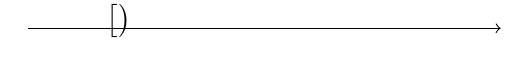
\begin{tikzpicture}
			\draw[->](-1,0)->(5,0); 
			\IntervalLR{-1}{1/2} 
			 \def\skipInterval{0.5cm}
			 \IntervalGRF{}{}{\big[}{3}
			 \IntervalLR{4}{4.8}
			\def\skipInterval{0.5cm} 
			 \IntervalGRF{\big)}{5}{}{}
		\end{tikzpicture}
	}\noindent 
	\choice{$A  = \left(3;5\right)$}
		{\True $A =  \left[3;5\right)$}
		{$A  = \left[3;5\right]$}
		 {$A = \left(3;5\right]$}
	\loigiai{ 
		Dễ thấy $A  = \left[3;5\right)$.
	 }
\end{ex}

% nguồn: MaHoaNH_TracNghiem_Lop10
\begin{ex}%[0D1B2-1]%[ma:0cfd13b7]
	 Cho tập hợp $X = \left[-3;5\right]$, biểu diễn tập hợp $X$ trên trục số ta được biểu diễn như sau (phần không bị gạch chéo)?
	\choice{ 
		 \True
		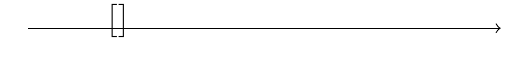
\begin{tikzpicture}
				 \draw[->](-1,0)->(5,0);
				 \IntervalLR{-1}{1/2}
				 \def\skipInterval{0.5cm}
				\IntervalGRF{}{}{\big[}{-3} 
				\IntervalLR{4}{4.8} 
				 \def\skipInterval{0.5cm}
				\IntervalGRF{\big]}{5}{}{} 
			\end{tikzpicture}
		 }{
		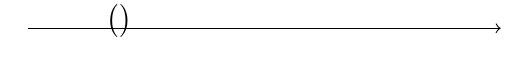
\begin{tikzpicture}
				\draw[->](-1,0)->(5,0); 
				 \IntervalLR{-1}{1/2}
				 \def\skipInterval{0.5cm}
				\IntervalGRF{}{}{\big (}{-3} 
				\IntervalLR{4}{4.8} 
				 \def\skipInterval{0.5cm}
				 \IntervalGRF{\big)}{5}{}{}
			\end{tikzpicture}
		}{ 
		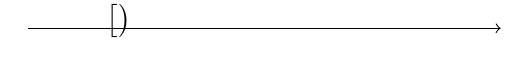
\begin{tikzpicture}
				\draw[->](-1,0)->(5,0); 
				 \IntervalLR{-1}{1/2}
				 \def\skipInterval{0.5cm}
				 \IntervalGRF{}{}{\big[}{-3}
				\IntervalLR{4}{4.8} 
				 \def\skipInterval{0.5cm}
				 \IntervalGRF{\big)}{5}{}{}
			\end{tikzpicture}
		}{ 
		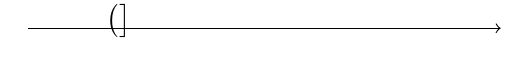
\begin{tikzpicture}
				 \draw[->](-1,0)->(5,0);
				 \IntervalLR{-1}{1/2}
				 \def\skipInterval{0.5cm}
				\IntervalGRF{}{}{\big  (}{-3}
				\IntervalLR{4}{4.8} 
				 \def\skipInterval{0.5cm}
				 \IntervalGRF{\big]}{5}{}{}
			\end{tikzpicture}
		 }
	 \loigiai{
	 $X = \left[-3;5\right]=\left\{x \in \mathbb{R} \mid -3\le x\le 5\right\}$ nên có biểu diễn trên trục số là
	\begin{center}
		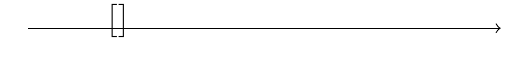
\begin{tikzpicture}
				\draw[->](-1,0)->(5,0); 
				\IntervalLR{-1}{1/2} 
				 \def\skipInterval{0.5cm}
				\IntervalGRF{}{}{\big[}{-3} 
				\IntervalLR{4}{4.8} 
				 \def\skipInterval{0.5cm}
				 \IntervalGRF{\big]}{5}{}{}
			\end{tikzpicture}
	\end{center}
	 }
\end{ex}


%%%%%%%%%%%%%%%% ĐÚNG/SAI %%%%%%%%%%%%%%%%

% nguồn: MaHoaNH_DungSai_Lop10
\begin{ex}%[0D1N2-1]%[ma:9215a246]
	Các câu sau là  đúng hay sai?
	 \choiceTF
		{\True Tập hợp các  ước nguyên dương của $24$ là $A=\{1;2;3;4;6;8;12;24\}$}
		{\True Tập hợp các chữ số trong số  $1113305$ là $B=\{0;1;3;5\}$}
		{Tập hợp các bội số của $5$ và  nhỏ hơn $30$ là $C=\{0;5;10;15;20;25;30\}$}
		{Tập hợp các nghiệm của phương  trình $x^2+9=0$ là $D=\{-3;3\}$}
	\loigiai{ 
	\begin{itemchoice}
		\itemch Tập hợp các ước  nguyên dương của $24$ là $A=\{1;2;3;4;6;8;12;24\}$.
		\itemch Tập hợp các chữ số trong số $1113305$ là $B=\{0;1;3;5\}$. 
		\itemch Tập hợp các bội số  của $5$ và nhỏ hơn $30$ là $C=\{0;5;10;15;20;25\}$.
		\itemch Tập hợp các nghiệm của phương trình  $x^2+9=0$ là $D=\varnothing$ (vì phương trình $x^2+9=0$ vô nghiệm).
	\end{itemchoice}
	} 
\end{ex}

% nguồn: MaHoaNH_DungSai_Lop10
\begin{ex}%[0D1H2-1]%[ma:8e7fb520]
	 Kí hiệu $T$ là tập hợp các học sinh của trường, $10$A là tập hợp các học sinh lớp $10$A của trường. Biết rằng An là một học sinh của lớp $10$A.
	 \choiceTF
		{\True An  $\in T$}
		{An $\subset 10$A} 
		{\True An $\in  10$A}
		 {$10$A $\in T$}
	 \loigiai{
		\begin{itemchoice}
			\itemch  An $\in T$.
			\itemch  An là một phần tử của tập hợp $X$.
			\itemch An  $\in 10A$.
			 \itemch $10$A là tập hợp con của tập hợp $T$.
		\end{itemchoice}
	 }
\end{ex}

% nguồn: MaHoaNH_DungSai_Lop10
\begin{ex}%[0D1H2-1]%[ma:9c349efe]
	Các  câu sau là đúng hay sai?
	 \choiceTF
		{Tập hợp các số tự nhiên lẻ là  $A=\left\{x\Big|x=2n, n\in\mathbb{N}\right\}$}
		{Tập hợp các nghiệm của phương trình $x+3y=1$ là $B=\left\{(x;y)\Big|x;y\in\mathbb{Z},  x+3y=1\right\}$}
		{\True Tập hợp các số nguyên tố nhỏ hơn $18$  là $C=\{2;3;5;7;11;13;17\}$}
		{\True Tập hợp các nghiệm của  phương trình $x^2+3x-4=0$ là $D=\{-4;1\}$}
	 \loigiai{
	\begin{itemchoice}
		\itemch Tập  hợp các số tự nhiên lẻ là $A=\left\{x\Big|x=2n+1, n\in\mathbb{N}\right\}$.
		\itemch Tập hợp các nghiệm của phương trình $x+3y=1$ là $B=\left\{(x;y)\Big|x;y\in\mathbb{R},  x+3y=1\right\}$.
		\itemch Tập hợp các số nguyên tố  nhỏ hơn $18$ là $C=\{2;3;5;7;11;13;17\}$.
		\itemch Ta có $x^2+3x-4=0 \Leftrightarrow \hoac{ &  x=-4 \\ & x=1.}$ \\
		 Vậy tập hợp các nghiệm của phương trình $x^2+3x-4=0$ là $D=\{-4;1\}$.
	\end{itemchoice}
	} 
\end{ex}

% nguồn: MaHoaNH_DungSai_Lop10
\begin{ex}%[0D1H2-1]%[ma:537923b5]
	Cho tập  hợp $X=\left\{-3;-1;0;1;3\right\}$.
	\choiceTF 
		{\True $-1$ là một phần tử của tập  hợp $X$}
		{\True Số tập hợp con của $X$ có $2$ phần tử là $10$} 
		{Tính chất đặc trưng của tập hợp $X$  là $X=\left\{x\in \mathbb{N}\mid 2x+1\le 5\right\}$}
		{\True Số tập con của tập hợp $X$ là $32$  tập hợp}
	 \loigiai{
		\begin{itemchoice}
			\itemch Ta có $-1\in X$ nên $-1$ là một phần tử của tập hợp  $X$.
			\itemch Tập hợp con của $X$ có $2$ phần  tử là
			 \[\left\{-4;-2\right\},\left\{-4;0\right\},\left\{-4;2\right\},\left\{-4;4\right\},\left\{-2;0\right\},\left\{-2;2\right\},\left\{-2;4\right\},\left\{0;2\right\},\left\{0;4\right\},\left\{2;4\right\}.
			 \]
			Vậy Số tập hợp con của $X$ có  $2$ phần tử là $10$.
			\itemch Tính chất đặc trưng  của tập hợp $X$ là $X=\left\{3x\mid \left|x\right|\le 1\text{ và }x\in \mathbb{Z}\right\}$.
			 \itemch
			\begin{itemize}
				\item Tập con của $X$ có $0$ phần tử có $1$ tập  hợp là tập $\varnothing$,
				\item Tập con của $X$ có $1$ phần  tử có $5$ tập hợp.
				\item Tập con của $X$ có $2$ phần tử có $10$  tập hợp.
				\item Tập  con của $X$ có $3$ phần tử có $10$ tập hợp.
				\item Tập con  của $X$ có $4$ phần tử có $5$ tập hợp.
				\item Tập con của $X$ có $5$ phần  tử có $1$ tập hợp.
			\end{itemize}
			Theo quy tắc cộng $1+5+10+10+5+1=32$  tập hợp.
		\end{itemchoice}
	 }
\end{ex}

% nguồn: MaHoaNH_DungSai_Lop10
\begin{ex}%[0D1V2-1]%[ma:b437d1ce]
	 Xét các phát biểu sau.
	\choiceTF 
		{\True Tập hợp $A=\{\left.  x\in \mathbb{Z}\right|1<x<10\}$ có $8$ phần tử}
		{\True Tập hợp $B=\left\{\left. x\in \mathbb{R}\right|x^2+x=0\right\}$ có $2$ phần tử} 
		{Tập hợp  $C=\left\{\left. x\in \mathbb{Q}\right|\left(x^2-1\right)(x-\sqrt{2})(2x+3)=0\right\}$ có $2$ phần tử}
		{\True Tập hợp $D=\{\left. n\in \mathbb{N}\right|-4<2n-1<5\}$ có  $3$ phần tử}
	\loigiai{ 
		\begin{itemchoice}
			\itemch $A=\{2; 3;  4; 5; 6; 7; 8; 9\}$.
			\itemch $B=\{-1;  0\}$.
			\itemch $C=\left\{\dfrac{-3}{2};-1; 1\right\}$. 
			\itemch $D=\{0; 1;  2\}$.
		\end{itemchoice}
	 }
\end{ex}

% nguồn: MaHoaNH_DungSai_Lop10
\begin{ex}%[0D1V2-1]%[ma:d132ee40]
	Cho  các tập hợp sau $A=\left\{\left. x\in \mathbb{R}\right|6x^2-7x+1=0\right\}$; $B=\left\{\left. x\in \mathbb{Z}\right||x|<1\right\}$; \break $C=\left\{\left. x\in \mathbb{Q}\right|x^2-4x+2=0\right\}$; $D=\left\{\left. x\in \mathbb{R}\right|x^2-4x+3=0\right\}$.
	\choiceTF 
		{Tập hợp $A$ là tập hợp  rỗng}
		{Tập  hợp $B$ là tập hợp rỗng}
		 {\True Tập hợp $C$ là tập hợp rỗng}
		 {Tập hợp $D$ là tập hợp rỗng}
	\loigiai{ 
		\begin{itemchoice}
			\itemch $A=\left\{\left. x\in  \mathbb{Z}\right|6x^2-7x+1=0\right\}$. \\
			Ta  có $6x^2-7x+1=0\Leftrightarrow \hoac{
			& x=1  \\
			 & x=\dfrac{1}{6}\notin \mathbb{Z}}\Rightarrow A=\{1\}\ne \varnothing$.
			 \itemch $B=\{\left. x\in \mathbb{Z}\right||x|<1\}\Rightarrow B=\{0\}\ne \varnothing. $
			 \itemch $C=\left\{\left. x\in \mathbb{Q}\right|x^2-4x+2=0\right\}$. \\
			Ta có $x^2-4x+2=0\Leftrightarrow \hoac{ 
			& x=2-\sqrt{2}\notin \mathbb{Q}  \\
			& x=2+\sqrt{2}\notin \mathbb{Q}}\Rightarrow  C=\varnothing$.
			\itemch  $D=\left\{\left. x\in \mathbb{R}\right|x^2-4x+3=0\right\}$.\\
			Ta  có $x^2-4x+3=0\Leftrightarrow \hoac{
			& x=1 \\ 
			& x=3}\Rightarrow D=\left\{\infty  1; 3\right\}\ne \varnothing$.
		\end{itemchoice}
	 }
\end{ex}

% nguồn: MaHoaNH_DungSai_Lop10
\begin{ex}%[0D1V2-1]%[ma:cd833910]
	Cho các  tập hợp
	$A=\{x\in\mathbb{Z}|\left|  x\right|<1\}$; $B=\left\{ x\in\mathbb{Z}\big|\,6x^2-7x+1=0\right\}$;\\
	 $C=\left\{ x\in\mathbb{Q}\big|\,x^2-4x+2=0\right\}$; $D=\left\{ x\in\mathbb{N}\big|\,x^2-4x+3=0\right\}$.
	\choiceTF 
		{Tập hợp  $A$ có $2$ phần tử}
		{\True Tập hợp $B$ có $1$ phần tử} 
		{Tập hợp $C$ có $3$  phần tử}
		{\True Tập hợp  $D$ có $2$ phần tử}
	 \loigiai{
		\begin{itemchoice}
			\itemch $ A=\{x\in\mathbb{Z}\big|\, |x|<1\}\Rightarrow A=\{0\}$. 
			\itemch  $ B=\left\{ x\in\mathbb{Z}\big| 6x^2-7x+1=0\right\}$.\\
			Ta có  $ 6x^2-7x+1=0\Leftrightarrow\hoac{
			&x=1\\&x=\dfrac{1}{6}\notin\mathbb{Z}}\Rightarrow  B=\{1\}$.
			\itemch  $ C=\left\{ x\in\mathbb{Q}\big|x^2-4x+2=0\right\}$.\\
			Ta  có $x^2-4x+2=0\Leftrightarrow\hoac{
			&x=2-\sqrt{2}\notin\mathbb{Q}\\&x=2+\sqrt{2}\notin\mathbb{Q}.}\Rightarrow  C=\varnothing$.
			\itemch $ D=\left\{  x\in\mathbb{N}\big|x^2-4x+3=0\right\}$.\\
			Ta  có $x^2-4x+3=0\Leftrightarrow\hoac{
			&  x=1\\
			& x=3}\Rightarrow D=\left\{ 1;3\right\}$. 
		\end{itemchoice}
	} 
\end{ex}

% nguồn: MaHoaNH_DungSai_Lop10
\begin{ex}%[0D1V2-1]%[ma:161eac9d]
	 Cho các tập hợp sau: A các số nguyên tố nhỏ hơn 11; $B=\left\{\left. x\in \mathbb{R}\right|3x^2-4x+1=0\right\}$;
	$C=\left\{\left. x\in  \mathbb{N}\right|\left(x^2-5x+6\right)\left(2x+1\right)=0\right\}$; $D=\{\left. x\in \mathbb{Z}\right|\left|x+1\right|<3\}$.
	 \choiceTF
		{\True Tập hợp $A$ có $4$ phần tử} 
		{Tập hợp $B$ có  $3$ phần tử}
		{Tập hợp  $C$ có $3$ phần tử}
		{\True Tập  hợp $D$ có $3$ phần tử}
	 \loigiai{
		\begin{itemchoice}
			\itemch Ta  có các số nguyên tố nhỏ hơn $11$ là $2$; $3$; $5$; $7$. \\
			Vậy $A=\{2; 3; 5; 7\}$. 
			\itemch Ta có $3x^2-4x+1=0\Leftrightarrow \hoac{ 
			&x=1\in \mathbb{R} \\ 
			 &x=\dfrac{1}{3}\in \mathbb{R}.}$ \\
			Vậy $B=\left\{\dfrac{1}{3};  1\right\}$.
			 \itemch Ta có $\left(x^2-5x+6\right)\left(2x+1\right)=0\Leftrightarrow \hoac{
			& x^2-5x+6=0 \\ 
			& 2x+1=0}\Leftrightarrow  \hoac{
			 & x=2\in \mathbb{N} \\
			& x=3\in \mathbb{N}  \\
			&  x=\dfrac{-1}{2}\notin \mathbb{N}.} $\\
			Vậy  $C=\left\{2; 3\right\}$.
			 \itemch Ta có $\heva{
			&x\in \mathbb{Z}  \\
			 &|x+1|<2}\Rightarrow \hoac{
			&x=-2  \\
			 &x=-1 \\
			 &x=0.} $\\
			Vậy $D=\{-2;-1; 0\}$. 
		\end{itemchoice}
	} 
\end{ex}

% nguồn: MaHoaNH_DungSai_Lop10
\begin{ex}%[0D1V2-1]%[ma:388b7f00]
	Cho các tập hợp sau $A=\left\{\left. x\in \mathbb{Q}\right|x^2-x-6=0\right\}$; $B=\left\{\left.  x\in \mathbb{Z}\right|x^4-11x^2+18=0\right\}$; \break $C=\left\{\left. x\in \mathbb{N}\right|\left(x^2-3x-10\right)\left(5x^3-6x^2+x\right)=0\right\}$; $D=\{\left. x\in \mathbb{Z}\right|-2<3x+7\le 10\}$.
	\choiceTF 
		 {\True Tập hợp $A$ có $2$ phần tử}
		{Tập hợp  $B$ có $3$ phần tử}
		{Tập  hợp $C$ có $2$ phần tử}
		{\True Tập hợp $D$  có $4$ phần tử}
	\loigiai{ 
		\begin{itemchoice}
			\itemch Ta có $x^2-x-6=0\Leftrightarrow  \hoac{
			 &x=-2\in \mathbb{Q} \\
			&x=3\in \mathbb{Q}.}$ \\ 
			 Vậy $A=\{-2; 3\}$.
			\itemch Ta có $x^4-11x^2+18=0\Leftrightarrow  \hoac{
			 &x^2=2 \\
			&x^2=9}\Leftrightarrow \hoac{ 
			&x=\sqrt{2}\notin  \mathbb{Z} \\
			 &x=-\sqrt{2}\notin \mathbb{Z} \\
			 &x=3\in \mathbb{Z} \\
			&x=-3\in  \mathbb{Z}.}$ \\
			Vậy $B=\{-3;  3\}$.
			\itemch Ta  có $\left(x^2-3x-10\right)\left(5x^3-6x^2+x\right)=0\Leftrightarrow \hoac{
			 &x^2-3x-10=0 \\
			 &5x^3-6x^2+x=0}\Leftrightarrow \hoac{
			&x=5\in \mathbb{N}  \\
			&x=-2\notin  \mathbb{N} \\
			 &x=0\in \mathbb{N} \\
			&x=1\in  \mathbb{N} \\
			 &x=\dfrac{1}{5}\notin \mathbb{N}.}$\\
			Vậy  $C=\left\{0; 1; 5\right\}$.
			\itemch Ta có $-2<3x+7\le  10\Leftrightarrow-3<x\le 1$. \\
			Mà $x\in  \mathbb{Z}\Rightarrow x\in D=\{-2;-1; 0; 1\}$.
		\end{itemchoice}
	} 
\end{ex}


%%%%%%%%%%%%%%%% TRẢ LỜI NGẮN %%%%%%%%%%%%%%%%

% nguồn: MaHoaNH_TraLoiNgan_Lop10
\begin{bt}%[0D1V2-1]%[ma:26c652e7]
	Xác định số phần tử của  tập hợp $ X=\left\{ n\in\mathbb{N}\big|n\,\vdots\,4\,,\,n<2017\right\}$.
	 \shortans{505}
	\loigiai{ 
		Tập hợp $ X$ gồm các phần tử là những số tự nhiên nhỏ hơn $ 2017$ và chia  hết cho $ 4$.\\
		Từ $ 0$ đến $ 2015$ có $ 2016$ số tự nhiên, ta thấy cứ $ 4$ số tự nhiên liên tiếp sẽ có duy nhất một số chia hết cho $ 4$. Suy ra có $ 504$ số tự nhiên chia hết cho  $ 4$ từ $ 0$ đến $ 2015$. Hiển nhiên $ 2016\,\vdots\,4$.\\
		 Vậy có tất cả $ 505$ số tự nhiên nhỏ hơn $ 2017$ và chia hết cho $ 4$.
	 }
\end{bt}

% nguồn: MaHoaNH_TraLoiNgan_Lop10
\begin{bt}%[0D1V2-1]%[ma:f7c72907]
	Trong một đợt phát động quyên góp sách, vở để giúp đỡ học sinh có hoàn cảnh khó khăn của trường THPT Triệu Sơn 2, lớp 10B2  có 30 học sinh tham gia quyên góp vở, 29 học sinh quyên góp sách. Biết rằng, tất cả học sinh trong lớp 10B2 đều tham gia quyên góp, trong đó có 14 học sinh quyên góp cả sách và vở. Hỏi lớp 10B2 có tất cả bao nhiêu học sinh?
	\shortans{45} 
	\loigiai{ 
		Gọi $n(S)$ là số HS quyên góp sách, $n(V)$ là số HS quyên góp  vở.\\
		$n(S)=29$,  $n(V)=30$.\\
		Số HS quyên góp cả sách và vở là $n(S\cap  V)=14$.\\
		Vì tất cả học sinh đều tham gia quyên góp nên số học sinh  của lớp là $n(S\cup V)$.\\
		$n(S\cup V)=n(S)+n(V)-n(S\cap V)=29+30-14=45$ (học sinh). 
	} 
\end{bt}

% nguồn: MaHoaNH_TraLoiNgan_Lop10
\begin{bt}%[0D1V2-1]%[ma:874a67ef]
	Cho tập $ X=\left\{ x\in\mathbb{R}|\left(x^2-4\right)\left(x-1\right)=0\right\}$. Tính tổng  $ S$ các phần tử của tập $ X$.
	 \shortans{1}
	 \loigiai{
		Các phần tử  của tập hợp $ X$ là các nghiệm thực của phương trình $\left(x^2-4\right)\left(x-1\right)=0$.\\
		Ta có  $\left(x^2-4\right)\left(x-1\right)=0\Leftrightarrow\hoac{
		&x^2-4=0\\ 
		&  x-1=0}\Leftrightarrow\hoac{
		&  x=\pm\ 2\\
		& x=1.}$\\ 
	Do  đó $ S=2+\left(-2\right)+1=1$.}
\end{bt}

% nguồn: MaHoaNH_TraLoiNgan_Lop10
\begin{bt}%[0D1V2-1]%[ma:c49376cc]
	Tìm số phần tử của tập hợp $ A=\left\{ x\in\mathbb{R}\big|  \left(x-1\right)\left(x+2\right)\left(x^3-4x\right)=0\right\}$.
	\shortans{4} 
	 \loigiai{
		$\left(x-1\right)\left(x+2\right)\left(x^3-4x\right)=0$$\Leftrightarrow\hoac{ 
		&  x-1=0\\
		&  x+2=0\\
		 &x^3-4x=0}\Leftrightarrow\hoac{
		&  x=1\\
		 & x=-2\\
		& x=0\\ 
		&  x=2.}$\\
	$\Rightarrow A=\left\{ 1;-2;0;2\right\}$. Vậy $ A$ có  $4$ phần tử.}
\end{bt}

% nguồn: MaHoaNH_TraLoiNgan_Lop10
\begin{bt}%[0D1V2-1]%[ma:9bf3cdd5]
	Cho tập $ X=\left\{ x\in\mathbb{N}|\left(x^2-4\right)\left(x-1\right)\left(2x^2-7x+3\right)=0\right\}$. Tính  tổng $ S$ các phần tử của $ X$.
	\shortans{6} 
	\loigiai{ 
		 Ta có $\left(x^2-4\right)\left(x-1\right)\left(2x^2-7x+3\right)=0\Leftrightarrow\hoac{
		 &x^2-4=0\\
		 & x-1=0\\
		&  2x^2-7x+3=0}\Leftrightarrow\hoac{
		& x=\pm  2\\
		& x=1\\ 
		 & x=3\\
		 & x=\dfrac{1}{2}.}$\\
		Vì $ x\in\mathbb{N}$ nên $  X=\left\{ 1;2;3\right\}$.\\
	Vậy tổng $  S=1+2+3=6$.}
\end{bt}

% nguồn: MaHoaNH_TraLoiNgan_Lop10
\begin{bt}%[0D1V2-1]%[ma:00aa5e91]
	Tập  hợp $A=\left\{\left. x\in\mathbb{N}\right|\left(x-1\right)\left(x+2\right)\left(x^3+4x\right)=0\right\}$ có bao nhiêu phần tử?
	 \shortans{2}
	\loigiai{ 
		 Ta có $\left(x-1\right)\left(x+2\right)\left(x^3+4x\right)=0\Leftrightarrow x\left(x-1\right)\left(x+2\right)\left(x^2+4\right)=0$\\
		$\Leftrightarrow\hoac{ 
		&  x=0\\
		&  x-1=0\\
		& x+2=0}\Leftrightarrow\hoac{ 
		&  x=1\\
		&  x=-2\\
		 & x=0.}$\\
		Vì $x\in\mathbb{N}$ nên chọn $x=0$; $x=1$. Vậy $A=\left\{ 0;1\right\}$ $\Rightarrow  $ tập $A$ có hai phần tử.
	 }
\end{bt}

% nguồn: MaHoaNH_TraLoiNgan_Lop10
\begin{bt}%[0D1V2-1]%[ma:1a8e2a1d]
	Lớp 10D có $15$ học sinh giỏi Toán, $18$ học sinh  giỏi Anh, $20$ học sinh giỏi Văn, $6$ học sinh giỏi cả Toán và Văn, $10$ học sinh giỏi cả Toán và Anh, $7$ học sinh giỏi cả Văn và Anh, $3$ học sinh giỏi cả ba môn Toán, Văn, Anh. Số học sinh lớp 10D là bao nhiêu?
	\shortans{33} 
	\loigiai{ 
		\begin{center}
			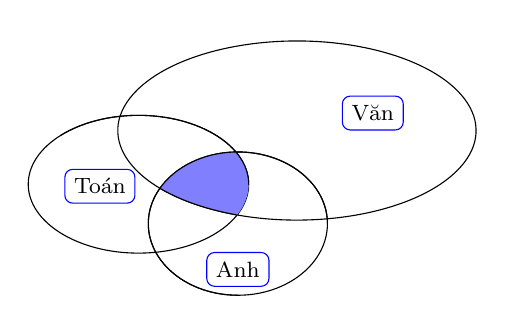
\begin{tikzpicture}[font=\footnotesize,line join=round,line cap=round,>=stealth]
					 \tikzset{s/.style={draw=blue,rounded corners=1mm,rectangle}}
					 \def\a{3.5}
					\def\b{0.55*\a} 
					\def\c{0.65*\a} 
					 \def\e{0.5*\c}
					 \def\f{0.5*\c}
					\def\g{0.4*\c} 
					 \def\m{0.4*\a}
					\def\n{0.25*\a} 
					\fill[white,draw=black](60:{\a}  and {\b}) arc (60:450:{\c} and {\e})
						(1,-0.5) arc (0:360:  {\f} and {\g})
						(0,0)  arc (0:360: {\m} and {\n});
					\begin{scope}
						 \clip (1,-0.5) arc (0:360: {\f} and {\g});
						\clip (0,0) arc  (0:360: {\m} and {\n});
						\fill[blue!50,draw=black](60:{\a} and  {\b}) arc (60:450:{\c} and {\e});
					\end{scope}
					 \draw
						 (60:{\a} and {\b})++(80:-1) node[s,above]{Văn}
						(0,0) arc (0:135:  {\m} and {\n})++(120:-1) node[s,above]{Toán}
						(1,-0.5)  arc (0:270: {\f} and {\g})++(-90:-.55) node[s,below]{Anh};
				\end{tikzpicture}
		\end{center}
		Từ sơ đồ Ven ta có 
		\begin{itemize}
			\item Số học sinh chỉ giỏi Văn và Toán  là $6-3=3$ (học sinh).
			\item Số học sinh chỉ giỏi Văn và Anh  là $7-3=4$ (học sinh).
			\item Số học sinh chỉ giỏi Toán và Anh là  $10-3=7$ (học sinh).
		\end{itemize}
		 Khi đó ta có
		\begin{itemize}
			 \item Số học sinh chỉ giỏi Toán là $15-3-3-7=2$ (học sinh).
			\item Số học  sinh chỉ giỏi Văn là $20-3-3-4=10$ học sinh).
			\item Số học sinh chỉ giỏi  Anh là $18-3-4-7=4$ (học sinh).
		\end{itemize}
		 Vậy tổng số học sinh lớp 10D là $3+(3+4+7)+(2+10+4)=33$ (học sinh).
	 }
\end{bt}


%%%%%%%%%%%%%%%% TỰ LUẬN %%%%%%%%%%%%%%%%

% nguồn: MaHoaNH_TuLuan_Lop10
\begin{bt}%[0D1H2-1]%[ma:2e3346e6]
	Viết lại các tập hợp sau  bằng cách chỉ rõ tính chất đặc trưng của các phần tử
	\begin{enumerate}[a)]
		\item $A =  \{0; 1; 2; 3; 4\}$.
		 \item $B = \{9; 36; 81; 144\}$.
	\end{enumerate}
	\loigiai{ 
		\begin{enumerate}[a)]
			\item Ta nhận thấy các phần tử của tập hợp $A$  là các số tự nhiên và nhỏ hơn $5$.\\
			Do đó $A = \{x \in \mathbb{N} \mid x  < 5\}$.
			\item Ta có $9 = 3^2$; $ 36 = 6^2$; $ 81 = 9^2$; $ 144 = 12^2$ và các số $3; 6; 9;  12 $ đều là bội của $3$.\\
			Do đó ta viết lại tập hợp $B$ bằng cách chỉ ra tính chất  đặc trưng là \linebreak $B = \{(3k)^2 \mid k \in \mathbb{N}^*; k \leq 4\}$.
		\end{enumerate}
	} 
\end{bt}

% nguồn: MaHoaNH_TuLuan_Lop10
\begin{bt}%[0D1H2-1]%[ma:be82e47e]
	Việt lại các tập hợp sau bằng cách liệt kê  các phần tử
	\begin{enumerate}[a)]
		\item  $A = \{x \in \mathbb{R} \mid 2x^2 - 5x + 3 = 0\}$.
		\item $B = \{x \in \mathbb{N}  \mid (9 - x^2)(x^2 - 3x + 2) = 0\}$.
		\item $C = \{x \in \mathbb{Q} \mid (5 - x^2)(x^2 - 5x  + 6) = 0\}$.
	\end{enumerate}
	 \loigiai{
		\begin{enumerate}
			\item Ta có $2x^2 - 5x + 3 = 0 \Leftrightarrow \hoac{& x  = 1 \in \mathbb{R}\\& x = \dfrac{3}{2} \in \mathbb{R}} \Rightarrow A = \left\{1; \dfrac{3}{2}\right\}$.
			\item Ta có $(9 - x^2)(x^2 - 3x + 2) = 0 \Leftrightarrow \hoac{& 9 - x^2 = 0\\& x^2 - 3x + 2 = 0} \Leftrightarrow \hoac{& x = -3\\& x = 3\\& x  = 1\\& x = 2.}$\\
			Vì $x \in \mathbb{N}$ nên $B = \{1; 2;  3\}$.
			\item Ta có $(5 - x^2)(x^2 - 5x + 6) = 0 \Leftrightarrow \hoac{& 5 -  x^2 = 0\\& x^2 - 5x + 6 = 0} \Leftrightarrow \hoac{& x = \pm \sqrt{5}\\& x = 3\\& x = 2.}$\\
			Vì $x \in  \mathbb{Q}$ nên $C = \{2; 3\}$.
		\end{enumerate}
	 }
\end{bt}

% nguồn: MaHoaNH_TuLuan_Lop10
\begin{bt}%[0D1H2-1]%[ma:2a9c1964]
	Viết lại các tập hợp sau bằng cách liệt kê các phần tử của nó 
	\begin{enumerate}[a)]
		\item $A = \{x \in \mathbb{R} \mid (2x^2 - 5x +  3)(x^2 - 4x + 3) = 0\}$.
		\item  $B = \{x \in \mathbb{N} \mid (2x^2 - 5x + 3)(x^2 - 4x + 3) = 0\}$.
		\item $C = \{x \in \mathbb{N} \mid x < 5\}$. 
	\end{enumerate}
	 \loigiai{
		\begin{enumerate}[a)]
			\item Ta có $(2x^2 - 5x + 3)(x^2 - 4x + 3) = 0 \Leftrightarrow \hoac{& 2x^2 - 5x + 3 = 0\\ &x^2 - 4x + 3 = 0} \Leftrightarrow \hoac{& x = 1\\& x = \dfrac{3}{2}\\& x = 1\\& x =  3.}$\\
			Vì $x \in \mathbb{R}$ nên $A =  \left\{1; \dfrac{3}{2}; 3 \right\}$.
			\item Ta có $(2x^2 - 5x + 3)(x^2 - 4x + 3) = 0 \Leftrightarrow \hoac{& 2x^2 - 5x + 3 = 0\\&  x^2 - 4x + 3 = 0} \Leftrightarrow \hoac{& x = 1\\& x = \dfrac{3}{2}\\& x = 1\\& x = 3.}$\\
			Vì $x \in \mathbb{N}$ nên $B  = \{1; 3\}$.
			\item Ta  có $x < 5$ và $x \in \mathbb{N}$ nên $x \in \{0; 1; 2; 3; 4\}$. Vậy $C = \{0; 1; 2; 3; 4\}$.
		\end{enumerate}
	 }
\end{bt}

% nguồn: MaHoaNH_TuLuan_Lop10
\begin{bt}%[0D1B2-1]%[ma:1d78e4f8]
	Viết lại tập hợp sau bằng cách liệt kê các phần  tử.
	$$A=\left\{ x\in \mathbb{Q}|  \, (2x^2-1)(2x^2-3x-5)=0\right\}.$$
	\loigiai{ 
		 Ta có $(2x^2-1)(2x^2-3x-5)=0\Leftrightarrow \hoac{&2x^2-1=0\\ &2x^2-3x-5=0 }\Leftrightarrow \hoac{&x=\pm \dfrac{\sqrt{2}}{2}\notin \mathbb{Q}\\&x=-1\\&x=\dfrac{5}{2}.}$\\
		 Vậy $A=\left\{ -1;\dfrac{5}{2}\right\} $.
	} 
\end{bt}

% nguồn: MaHoaNH_TuLuan_Lop10
\begin{bt}%[0D1B2-1]%[ma:9eda731e]
	Cho hai  tập hợp $A=\left\{ x \in \mathbb{Z} \ \mid dle | \ (2x^2-x-3)(x^2-4) = 0 \right\}$ và $B=\left\{ x \in \mathbb{N} \ \mid dle | \ x<4 \right\}$. Viết lại các tập hợp $A$ và $B$ bằng cách liệt kê các phần tử.
	 \loigiai{
		 Ta có
		\[\left(2x^2-x-3\right)\left(x^2-4\right)=0  \Leftrightarrow \hoac{& 2x^2-x-3=0\\& x^2-4=0} \Leftrightarrow \hoac{& (x+1)(2x-3)=0\\& x^2=4} \Leftrightarrow \hoac{& x=-1\\& x=\dfrac{3}{2}\\& x=\pm 2}\]
		Do $x \in \mathbb{Z}  \Rightarrow x \in \left\{ -2;-1;2 \right\}$ hay $A=\left\{ -2;-1;2 \right\}$.\\
		 $B=\left\{ x \in \mathbb{N} \ \mid dle | \ x<4 \right\}=\left\{0;1;2;3\right\}$.
	} 
\end{bt}

% nguồn: MaHoaNH_TuLuan_Lop10
\begin{bt}%[0D1Y2-1]%[ma:dd4a60c5]
	Cho $D=\{n  \in \mathbb{N} \mid n$ là số nguyên tố, $5<n<20\}$.
	\begin{enumEX}{1}
		\item Viết tập hợp $D$ bằng cách liệt  kê các phần tử. Tập hợp $D$ có bao nhiêu phần tử?
		\item  Dùng kí hiệu $\in, \notin$ để viết câu trả lời cho câu hỏi sau: Trong các số $5$; $12$; $17$; $18$, số nào thuộc tập $D$, số nào không thuộc tập $D$?
	\end{enumEX}
	\loigiai{ 
		\begin{enumEX}{1}
			\item $D=\{7; 11; 13; 17; 19\}$. Tập hợp $D$ có $5$ phần tử. 
			\item $5 \notin D$; $12 \notin D$; $17 \in  D$; $18 \notin D$.
		\end{enumEX}
	 }
\end{bt}

% nguồn: MaHoaNH_TuLuan_Lop10
\begin{bt}%[0D1B2-1]%[ma:4ed8e967]
	Cho tập hợp $ A=\{1,2,3,4\}  $.
	\begin{enumEX}{2}
		\item Liệt kê tất cả các  tập hợp con có $ 3 $ phần tử của $ A $.
		\item Liệt kê tất cả tập con có $ 2 $ phần tử  của $ A $.
		\item Liệt kê tất  cả các tập con của $ A $.
	\end{enumEX}
	 \loigiai{
		\begin{enumEX}{1}
			 \item $ A_1=\{1,2,3\};A_2=\{1,2,4\}; A_3=\{1,3,4\}; A_4=\{2,3,4\}$
			\item $ B_1=\{1,2\}; B_2=\{1,3\}; B_3=\{1,4\};  B_4=\{2,3\}; B_5=\{2,4\}; B_6=\{3,4\} $.
			\item $ C_1=\{1\}; C_2=\{2\}; C_3=\{3\}; C_4=\{4\};  C_5=A; C_6=\emptyset; A_1=\{1,2,3\};A_2=\{1,2,4\}; A_3=\{1,3,4\}; A_4=\{2,3,4\}; B_1=\{1,2\} B_2=\{1,3\}; B_3=\{1,4\}; B_4=\{2,3\}; B_5=\{2,4\}; B_6=\{3,4\} $.
		\end{enumEX}
	 }
\end{bt}

% nguồn: MaHoaNH_TuLuan_Lop10
\begin{bt}%[0D1K2-1]%[ma:d1db4126]
	Viết mỗi tập hợp sau bằng cách nêu tính chất đặc  trưng.
	\begin{enumEX}{2}
		\item  $A=\{2;3;5;7\}$.
		\item  $B=\{-3;-2;-1;0;1;2;3\}$.
		 \item $C=\{-5;0;5;10\}$.
		 \item $D=\{1;2;3;4;6;9;12;18;36\}$.
	\end{enumEX}
	\loigiai{ 
		\begin{enumerate}
			 \item $A=\left\{x\in \mathbb{R}\big|\right. x$ nguyên tố và $\left.x<10\right\}$.
			\item $B=\left\{x\in  \mathbb{Z}\big||x|\leqslant 3 \right\}$.
			\item $C=\left\{x\in \mathbb{Z}\big| x\vdots 5,-5\leqslant  x\leqslant 10 \right\}$.
			\item $D=\left\{n\in \mathbb{N}\big|x \text{  là ước của } 36\right\}$.
		\end{enumerate}
	} 
\end{bt}

% nguồn: MaHoaNH_TuLuan_Lop10
\begin{bt}%[0D1B2-1]%[ma:173ca8c7]
	Viết các tập hợp  sau bằng phương pháp liệt kê.
	\begin{enumEX}{2}
		\item $ A=\{x  \in \mathbb{Q} | (2x-x^2)(2x^2-3x-2)=0 \} $.
		\item $ B=\{n \in \mathbb{N} |  3<n^2<30 \} $.
		\item $ C=\{x \in  \mathbb{R} | x^4-5x^2+6=0\} $.
		\item $  D=\{n \in \mathbb{Z} | 0<n^2<30\} $.
	\end{enumEX}
	\loigiai{ 
		\begin{enumEX}{1}
			\item $ (2x-x^2)(2x^2-3x-2)=0 \Leftrightarrow \hoac{&x=0\\&x=2\\&x=-\dfrac{1}{2}} $. Do $ x  \in \mathbb{Q} $ nên nhận hết ba nghiệm. Vậy $ A=\left\{0,-\dfrac{1}{2},2\right\} $.
			\item $ 3<n^2<30 \Leftrightarrow \hoac{& \sqrt{3} <n<\sqrt{30}\\&-\sqrt{30}<n<\-\sqrt{3}} $. Do $ n \in \mathbb{N} $ nên $ B=\{2,3,4,5\} $. 
			\item  $ x^4-5x^2+6=0 \Leftrightarrow \hoac{&x=\pm \sqrt{3}\\&x=\pm \sqrt{2}} $. Do $ x \in \mathbb{R} $ nên $ C=\{-\sqrt{3}, -\sqrt{2}, \sqrt{2}, \sqrt{3}\} $.
			\item $  0<n^2<30 \Leftrightarrow 0<n<\sqrt{30} $. Do $ n \in \mathbb{Z}$ nên $ D=\{1,2,3,4,5\} $.
		\end{enumEX}
	 }
\end{bt}

% nguồn: MaHoaNH_TuLuan_Lop10
\begin{bt}%[0D1B2-1]%[ma:2e2e7223]
	\begin{listEX}[1]
		\item Liệt kê các phần tử của mỗi  tập hợp sau
		\begin{center}
			$A=\{ x\in \mathbb{Z}  \mid -5<x\leq 2\}$ và
			$B=\{ x\in \mathbb{N}  \mid(2x-1)(x^2-6x+5)=0\}$.
		\end{center}\vspace{-1.5cm}
		\item Viết lại tập hợp sau bằng cách nêu tính chất đặc  trưng $C=\{ 0;6;12;18;24;30;36;42 \}$.
	\end{listEX}
	\loigiai{ 
		\begin{listEX}[1]
			\item 
			$A=\{-4;-3;-2;-1;0;1;2\}$.\\ 
			 $B=\{ 1;5\}$.
			\item $C=\{ 6k \mid k \in \mathbb{N}, k  \le 7 \}$.
		\end{listEX}
	 }
\end{bt}

% nguồn: MaHoaNH_TuLuan_Lop10
\begin{bt}%[CTST10]%[0D1B2-1]%[ma:a092b757]
	Viết các tập hợp sau  đây dưới chỉ ra tính chất đặc trưng cho các phần tử:
	\begin{enumerate}[a)]
		\item Tập  hợp $ A=\left\{1;2;3;6;9;18\right\} $;
		\item Tập hợp $ B $ các nghiệm của bất phương trình $ 2x+1>0  $;
		\item Tập  hợp $ C $ các nghiệm của phương trình $ 2x-y=6 $.
	\end{enumerate}
	\loigiai{ 
		\begin{enumerate}[a)]
			\item  Tập hợp $ A=\left\{1;2;3;6;9;18\right\} $.\\
			Ta có $ A=\left\{x\in \mathbb{N}\ \mid dle| \ x\text{ là  ước của } 18\right\} $.
			\item Tập hợp $ B $ các nghiệm của bất  phương trình $ 2x+1>0 $.\\
			Ta có $ B=\left\{x\in \mathbb{R}\ \mid  dle| \ 2x+1>0\right\} $.
			\item Tập hợp $ C $ các nghiệm của phương trình $  2x-y=6 $.\\
			Ta có $ C=\left\{(x;y)\ \mid dle| \  x,y \in \mathbb{R}, 2x-y=6\right\} $.
		\end{enumerate}
	 }
\end{bt}

% nguồn: MaHoaNH_TuLuan_Lop10
\begin{bt}%[CTST10]%[0D1B2-1]%[ma:1f9a4e09]
	Viết các tập hợp sau đây dưới dạng liệt kê  các phần tử:
	\begin{enumerate}[a)]
		\item $ A=\left\{x\in \mathbb{Z}\ \mid dle| \ |x|<5\right\}  $;
		\item $  B=\left\{x\in \mathbb{R}\ \mid dle| \ 2x^2-x-1=0\right\} $;
		\item $ C=\left\{x\in \mathbb{N}\ \mid dle| \ x \text{ có  hai chữ số}\right\} $.
	\end{enumerate}
	 \loigiai{
		\begin{enumerate}[a)]
			\item Ta có $ |x|<5 \Leftrightarrow  -5<x<5 $.\\
			Vì $ x\in \mathbb{Z} $  nên $ x\in \left\{ -4;-3;-2;-1;0;1;2;3;4\right\}$.\\
			Vậy  $ A=\left\{-4;-3;-2;-1;0;1;2;3;4\right\} $.
			\item Ta có $ 2x^2-x-1=0\Leftrightarrow \hoac{&x=1\\&x=-\dfrac{1}{2}.} $\\ 
			Vì $ x\in  \mathbb{R} $ nên $ x\in \left\{ -\dfrac{1}{2};1\right\}$.\\
			Vậy  $ B=\left\{-\dfrac{1}{2};1\right\} $.
			\item $ C=\left\{10;11;12;\ldots;99\right\} $. 
		\end{enumerate}
	 }
\end{bt}

% nguồn: MaHoaNH_TuLuan_Lop10
\begin{bt}%[0D1B2-1]%[ma:66d7b781]
	Trong các tập hợp sau đây, tập nào là  tập rỗng?
	\begin{enumerate}
		\item $A=\left\{{x\in  \mathbb{Z}\left|{|x|<1}\right.}\right\}$.
		\item $B=\left\{{x\in  \mathbb{R}\left|{x^2-x+1=0}\right.}\right\}$.
		 \item $C=\left\{{x\in \mathbb{Q}\left|{x^2-4x+2=0}\right.}\right\}$.
		 \item $D=\left\{{x\in \mathbb{Q}\left|{x^2-2=0}\right.}\right\}$.
		\item  $E=\left\{{x\in \mathbb{N}\left|{x^2+7x+12=0}\right.}\right\}$.
		 \item $F=\left\{{x\in \mathbb{R}\left|{x^2-4x+2=0}\right.}\right\}$.
	\end{enumerate}
	\loigiai{ 
		\begin{enumerate}
			\item $|x|<1\Leftrightarrow  x=0\in \mathbb{Z}$
			 \item $x^2-x+1=0$ pt vô nghiệm
			\item  $x^2-4x+2=0\Leftrightarrow x=2\pm \sqrt{2}\notin \mathbb{Q}$
			\item $x^2-2=0\Leftrightarrow  x=\pm\sqrt{2}\notin \mathbb{Q}$
			\item $x^2+7x+12=0\Leftrightarrow  \hoac{&x=-3\notin \mathbb{N}\\&x=-4\notin \mathbb{N}}$
			\item  $x^2-4x+2=0\Leftrightarrow x=2\pm \sqrt{2} \in \mathbb{R}$
		\end{enumerate}
	} 
\end{bt}

% nguồn: MaHoaNH_TuLuan_Lop10
\begin{bt}%[0D1K2-1]%[ma:dda14c13]
	Viết mỗi tập hợp sau bằng cách  liệt kê các phần tử của nó.
	\begin{enumerate}
		 \item $A=\left\{x\in \mathbb{R}\left|{\left(2x^2-5x+3\right)\left(x^2-4x+3\right)=0}\right.\right\}$.
		 \item $B=\left\{x\in \mathbb{R}\left|{\left(x^2-10x+21\right)\left(x^3-x\right)=0}\right.\right\}$.
		\item $C=\left\{x\in \mathbb{R}\left|{\left(6x^2-7x+1\right)\left(x^2-5x+6\right)=0}\right.\right\}$. 
		\item  $D=\left\{{x\in \mathbb{Z}\left|{2x^2-5x+3=0}\right.}\right\}$.
		 \item $E=\left\{{x\in \mathbb{N}\left|{x+3<4+2x;5x-3<4x-1}\right.}\right\}$.
		\item  $F=\left\{{x\in \mathbb{Z}\left|{|x+2|\le 1}\right.}\right\}$.
		\item  $G=\left\{{x\in \mathbb{N}\left|{x<5}\right.}\right\}$.
		 \item $H=\left\{{x\in \mathbb{R}\left|{x^2+x+3=0}\right.}\right\}$.
		\item $K=\left\{{x\in \mathbb{Q}\left|{x=\dfrac{1}{2^a}\le  \dfrac{1}{32},a\in \mathbb{N}}\right.}\right\}$.
	\end{enumerate}
	\loigiai{ 
		\begin{enumerate}
			\item $(2x^2-5x+3)(x^2-4x+3)=0\Leftrightarrow  \hoac{&2x^2-5x+3=0\\&x^2-4x+3=0}\Leftrightarrow\hoac{&x=\dfrac{3}{2}\\&x=1\\&x=3\\&x=1}\Rightarrow A=\left\{\dfrac{3}{2};1;3\right\}$.
			\item $(x^2-10x+21)(x^3-x)=0\Leftrightarrow \hoac{&x=7\\&x=3\\&x=0\\&x=1\\&x=-1}\Rightarrow B=\{-1;0;1;3;7\}$. 
			\item $(6x^2-7x+1)(x^2-5x+6)=0\Leftrightarrow \hoac{&x=1\\&x=\dfrac{1}{6}\\&x=3\\&x=2}\Rightarrow C=\left\{\dfrac{1}{6};1;2;3\right\}$. 
			\item  $2x^2-5x+3=0\Leftrightarrow \hoac{&x=1\\&x=\dfrac{3}{2}\notin \mathbb{Z}.}\Rightarrow D=\{1\}$.
			\item $x+3<4+2x\Leftrightarrow x>-1$.\\ 
			$5x-3<4x-1\Leftrightarrow x<2$. Mà $x\in \mathbb{N}\Rightarrow E=\{0;1\}$ 
			\item $|x+2|\le 1\Leftrightarrow -1\le x+2\le 1\Leftrightarrow -3\le x\le  -1$. Mà $x\in \mathbb{Z}\Rightarrow F=\{-3;-2;-1\}$.
			\item $x\in\mathbb{N}$, $x<5\Rightarrow G=\{0;1;2;3;4\}$ 
			\item $x^2+x+3=0$ (vô nghiệm) $\Rightarrow  H=\varnothing$.
			\item  $a\in\mathbb{N}$, $a=\{5;6;7;8;\ldots\}$. Vậy $Q= \left\{\dfrac{1}{32};\dfrac{1}{64};\dfrac{1}{128};\dfrac{1}{256};\ldots\right\} $
		\end{enumerate}
	} 
\end{bt}

% nguồn: MaHoaNH_TuLuan_Lop10
\begin{bt}%[0D1B2-1]%[ma:5185a59d]
	Viết các tập hợp sau bằng phương pháp nêu  ra tính đặc trưng.
	\begin{enumEX}{2}
		 \item $ A=\{1,2,3,4,5,6,7,8,9 \} $.
		\item $  B=\{0,2,4,6,8,10 \} $.
		\item $ C=\{-3,-2,-1,0,1,2,3\} $. 
		\item $ D=\{1,4,7,10,13,16,19\}  $.
		\item $ D=\{1,2,4,8,16,32,64,128,256,512\} $. 
		\item Tập hợp các  số chẵn.
		 \item Tập hợp các số lẻ.
		\item Đường phân giác trong của  $ \widehat{ABC} $.
		\item Đường tròn tâm $ I $, bán kính $ R  $.
		\item Đường tròn  đường kính $ AB $.
		\item $  A=\{-2,1,6,13,22,33,46,61\} $.
		\item $  A=\{3,8,24,35,48,63,80,99\} $.
		\item $ A=\left\{0\dfrac{1}{3},\dfrac{2}{9},\dfrac{3}{19},\dfrac{4}{33},\dfrac{5}{51},\dfrac{6}{73}\right\}  $.
		\item $ A=\left\{\dfrac{2}{3};1;\dfrac{10}{7},\dfrac{17}{9},\dfrac{26}{11}, \dfrac{37}{13},\dfrac{10}{3}\right\}  $.
	\end{enumEX}
	 \loigiai{
		\begin{enumEX}{2}
			\item $ A=\{x \in  \mathbb{N^*} | x<10\} $.
			\item $ B=\{x \in \mathbb{N} | x \text{ là số chẵn và  } x \le 10\} $ hoặc\\
			$ B=\{ 2x | x \in \mathbb{N}, x  \le 5\} $.
			\item $ C=  \{x \in \mathbb{Z} | -3\le x \le 3\} $ hoặc\\
			$ C =\{ x \in \mathbb{Z}| |x|\le 3\}  $.
			\item $ D=\{3n-2| n \in \mathbb{N^*}, n  \le 7 \} $.
			\item $ D=\{2^n  | n \in \mathbb{N}, n \le 9 \} $.
			\item $ E=\{2n | n \in \mathbb{Z}\} $. 
			\item $ F=\{2n+1 | n \in \mathbb{Z}\} $. 
			\item $ G=\{Bx | \widehat{ABx}=\widehat{CBx}, Bx \text{ nằm giữa hai tia } BA \text{  và } BC\}$.
			\item  $ H=\{M | IM=R\text{ cố định}\} $.
			\item $ T=\left\{ M |  \widehat{AMB}=90^\circ\right\} $.
			\item $  K=\{n^2-3 | n \in \mathbb{N}, 1\le n \le 8\} $.
			\item $ L=\{n^2-1 | n \in \mathbb{N}, 2\le n \le  10, n \ne 4\} $.
			\item $ M=\left\{\dfrac{n}{2n^2+1}|  n \in \mathbb{N}, n \le 6\right\} $.
			\item $ N=\left\{\dfrac{n^2+1}{2n+1}, n\in \mathbb{N^*}, n \le 7\right\}  $.
		\end{enumEX}
	} 
\end{bt}

% nguồn: MaHoaNH_TuLuan_Lop10
\begin{bt}%[0D1K2-1]%[ma:c4dca562]
	Viết mỗi tập hợp sau bằng cách chỉ rõ tính chất đặc trưng cho các phần tử  của nó:
	\begin{enumerate}
		 \item $A=\left\{{0;1;2;3;4}\right\}$.
		\item  $C=\left\{{-3;9;-27;81}\right\}$.
		 \item $D=\left\{{9;36;81;144}\right\}$.
		\item  $E=\left\{{2;3;5;7;11}\right\}$.
		 \item $F=\left\{{3;6;9;12;15}\right\}$.
		\item  $G=\left\{{0;3;8;15;24;35;48;63}\right\}$.
		\item $H=\left\{{1;\dfrac{1}{3};\dfrac{1}{9};\dfrac{1}{27};\dfrac{1}{81};\dfrac{1}{243}}\right\}$. 
		 \item $I=\left\{{\dfrac{1}{2};\dfrac{1}{6};\dfrac{1}{12};\dfrac{1}{20};\dfrac{1}{30}}\right\}$.
		\item  $J=\left\{{\dfrac{2}{3};\dfrac{3}{8};\dfrac{4}{15};\dfrac{5}{24};\dfrac{6}{35}}\right\}$.
		\item $K=\left\{{-4;-3;-2;-1;0;1;2;3;4;5}\right\}$. 
		\item $M=\left\{{1,\dfrac{2}{3},\dfrac{3}{5},\dfrac{4}{7},\dfrac{5}{9},\dfrac{6}{11},\dfrac{7}{13},\dfrac{8}{15}}\right\}$. 
		\item  $O=\left\{{0,\sqrt{3},2\sqrt{2},\sqrt{15},2\sqrt{6},\sqrt{35},4\sqrt{3},\sqrt{63}}\right\}$.
		\item $P=\left\{{0,\dfrac{1}{2},\dfrac{2}{3},\dfrac{3}{4},\dfrac{4}{5},\dfrac{5}{6},\dfrac{6}{7},\dfrac{7}{8},\dfrac{8}{9},\dfrac{9}{10}}\right\}$. 
		\item $Q=$ Tập tất cả các điểm  thuộc đường trung trực của đoạn thẳng $AB$.
		\item $R=$ Tập tất cả các điểm thuộc đường tròn tâm $I$ cho trước và có bán kính bằng $5$. 
	\end{enumerate}
	 \loigiai{
		\begin{enumerate}
			 \item $A=\{x\in\mathbb{N}|x\le 4\}$
			\item $0+4=4$, $4+4=8$, $8+4=12$, $12+4=16$. Suy ra  $B=\{x=k+4|k\in\mathbb{N},k\le 4\}$
			\item $(-3)^2=9$, $(-3)^3=-27$, $(-3)^4=81$. Suy  ra $C=\{x=(-3)^k|k\in\mathbb{N}, 2\le k\le 4\}$
			\item $9=(3\cdot 1)^2$, $36=(3\cdot 2)^2$,  $81=(3\cdot 3)^2$, $144=(3\cdot 4)^2$. Suy ra $D=\{x=(3k)^2|k\in\mathbb{N},1\le k\le 4\}$.
			\item  $2$, $3$, $5$, $7$, $11$ là các số nguyên tố
			\item $3=3\cdot 1$, $6=3\cdot  2$, $9=3\cdot 3$, $12=3\cdot 4$. Suy ra $F=\{x=3k| k\in\mathbb{N}, 1\le k\le 5\}$.
			\item $0^2+2\cdot 0=0$, $1^2+2\cdot 1=3$,  $2^2+2\cdot 2=8$, $3^2+2\cdot 3=15$, $4^2+2\cdot 4=24$, \ldots. Suy ra $G=\{x=k^2+2k|k\in\mathbb{N}, k\le 7\}$.
			\item  $H=\left\{x=\dfrac{1}{3^k}|k\in\mathbb{N}, k\le 5\right\}$
			\item $I=\left\{x=\dfrac{1}{k(k+1)}|k\in\mathbb{N},1\le  k\le 5\right\}$
			\item $J=\left\{x=\dfrac{k+1}{k^2+2k}|k\in\mathbb{N},1\le k\le  5\right\}$
			\item $K=\{x\in\mathbb{Z}|-4\le x\le  5\}$
			\item $M=\left\{x=\dfrac{k+1}{2k+1}|k\in\mathbb{N}, k\le 7\right\}$ 
			\item $O=\{x=\sqrt{k^2+2k}|k\in\mathbb{N},k\le 7\}$ 
			 \item $P=\left\{x=\dfrac{k}{k+1}|k\in\mathbb{N}, k\le 9\right\}$
			\item  $Q=\{M|MA=MB\}$
			\item $R=\{M|IM=5\text{với I  là điểm cố định}\}$
		\end{enumerate}
	} 
\end{bt}
